\documentclass{beamer} 
\mode<presentation>
{
  \usetheme{Warsaw} 
  \setbeamercovered{transparent}
  \setbeamertemplate{footline}[frame number]
}

\usepackage[english]{babel} 
\usepackage{graphicx}
\usepackage{pdfpages}
\usepackage{tikz} 
\usepackage[latin1]{inputenc}
\usepackage{times}
\usepackage[T1]{fontenc} 
\title[Research Proposal] % (optional, use only with long paper titles)
{NONLINEAR AND RATE-DEPENDENT HYSTERETIC ELECTRO MECHANICAL RESPONSES OF FERRO ELECTRIC MATERIALS}
 

\author [Sohrabi Mollayosuef, Amir] % (optional, use only with lots of authors)
{Amir Sohrabi Mollayosuef}

\institute[Texas A\&M University] % (optional, but mostly needed)
{ Department of Mechanical Engineering\\
  Texas A\&M University}

\date[16th December 2014] % (optional, should be abbreviation of conference
% name)
{A Presentation for Tire Mechanics and Material Group in Cooper Tire}

\subject{Computational Solid Mechanics}

\pgfdeclareimage[height=0.5cm]{university-logo}{../images/university-logo-filename}
\logo{\pgfuseimage{university-logo}}

\AtBeginSubsection[]
{
  \begin{frame}<beamer>{Outline}
    \tableofcontents[currentsection,currentsubsection]
  \end{frame}
}

\begin{document}

\begin{frame}
  \titlepage
\end{frame}

\begin{frame}{Outline}
  \tableofcontents
  % You might wish to add the option [pausesections]
\end{frame}

\section{Introduction} 

\subsection{Application of Piezoelectric Materials}

\begin{frame}{Application of Piezoelectric Materials}

     \begin{columns}[t] 
     \begin{column}[T]{5cm} 
       \begin{itemize} \itemsep8ex
  \item  Actuation \cite{Berner1999}
  \item  Sensing
   \item  Energy Harvesting \cite{roundy2004piezoelectric}
  \end{itemize} 
     \end{column}
     \begin{column}[T]{5cm} 
      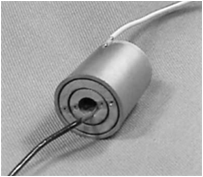
\includegraphics[height=2cm]{../images/telescpic_actuator_picture}\\
      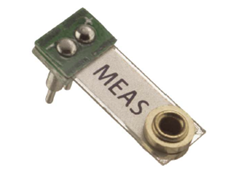
\includegraphics[height=2cm]{../images/piezeo_sensor}\\
      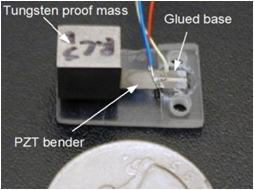
\includegraphics[height=2cm]{../images/piezeo_harvester}\\     
     \end{column}
     \end{columns}    
\end{frame}

\subsection{Introduction on Piezoelectricity}
\begin{frame}{Crystal Structure of PZT}
The origin of electromechanical coupling is polarization
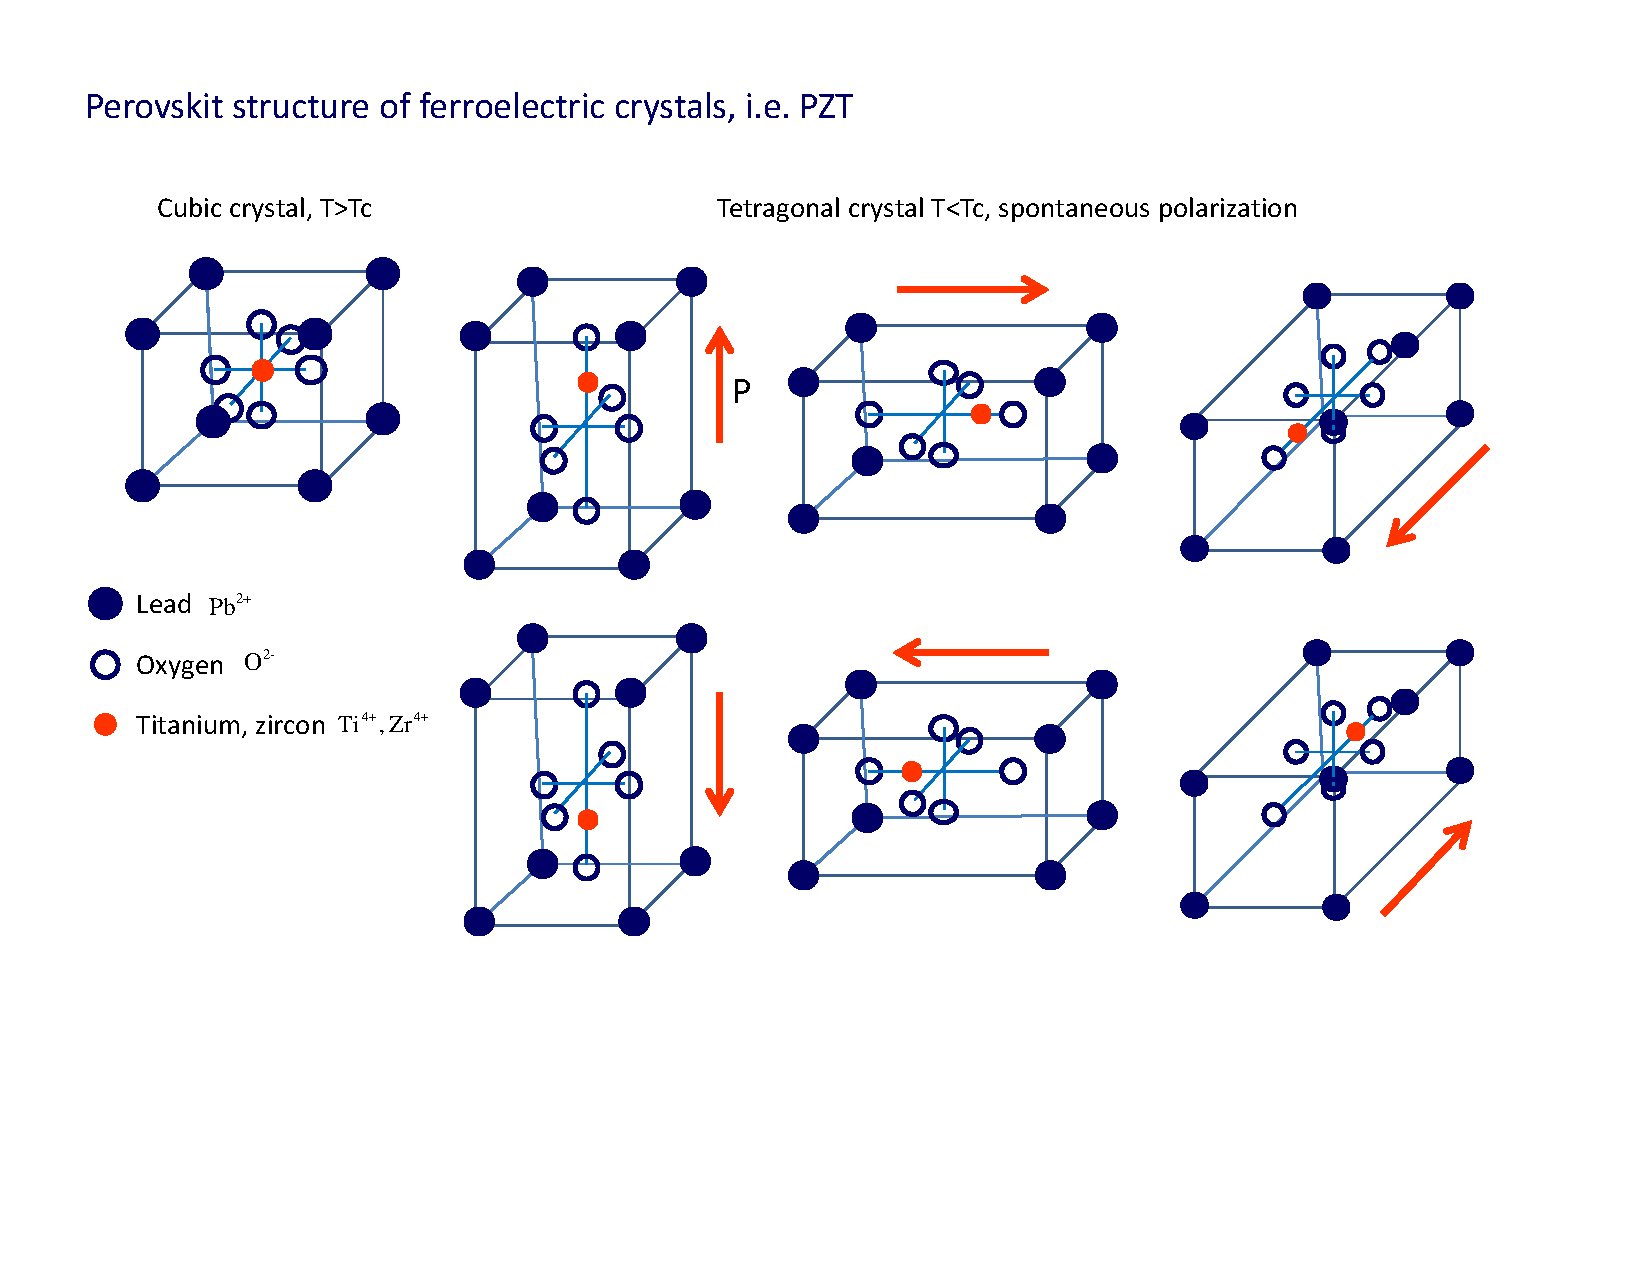
\includegraphics[height=7cm]{../images/piezo_electric_basics} \\ 
\end{frame} 

\begin{frame}{Polarization in the bulk material}
Each grain contain crystals with same structures and polarization.
Overall polarization is zero in virgin sample.
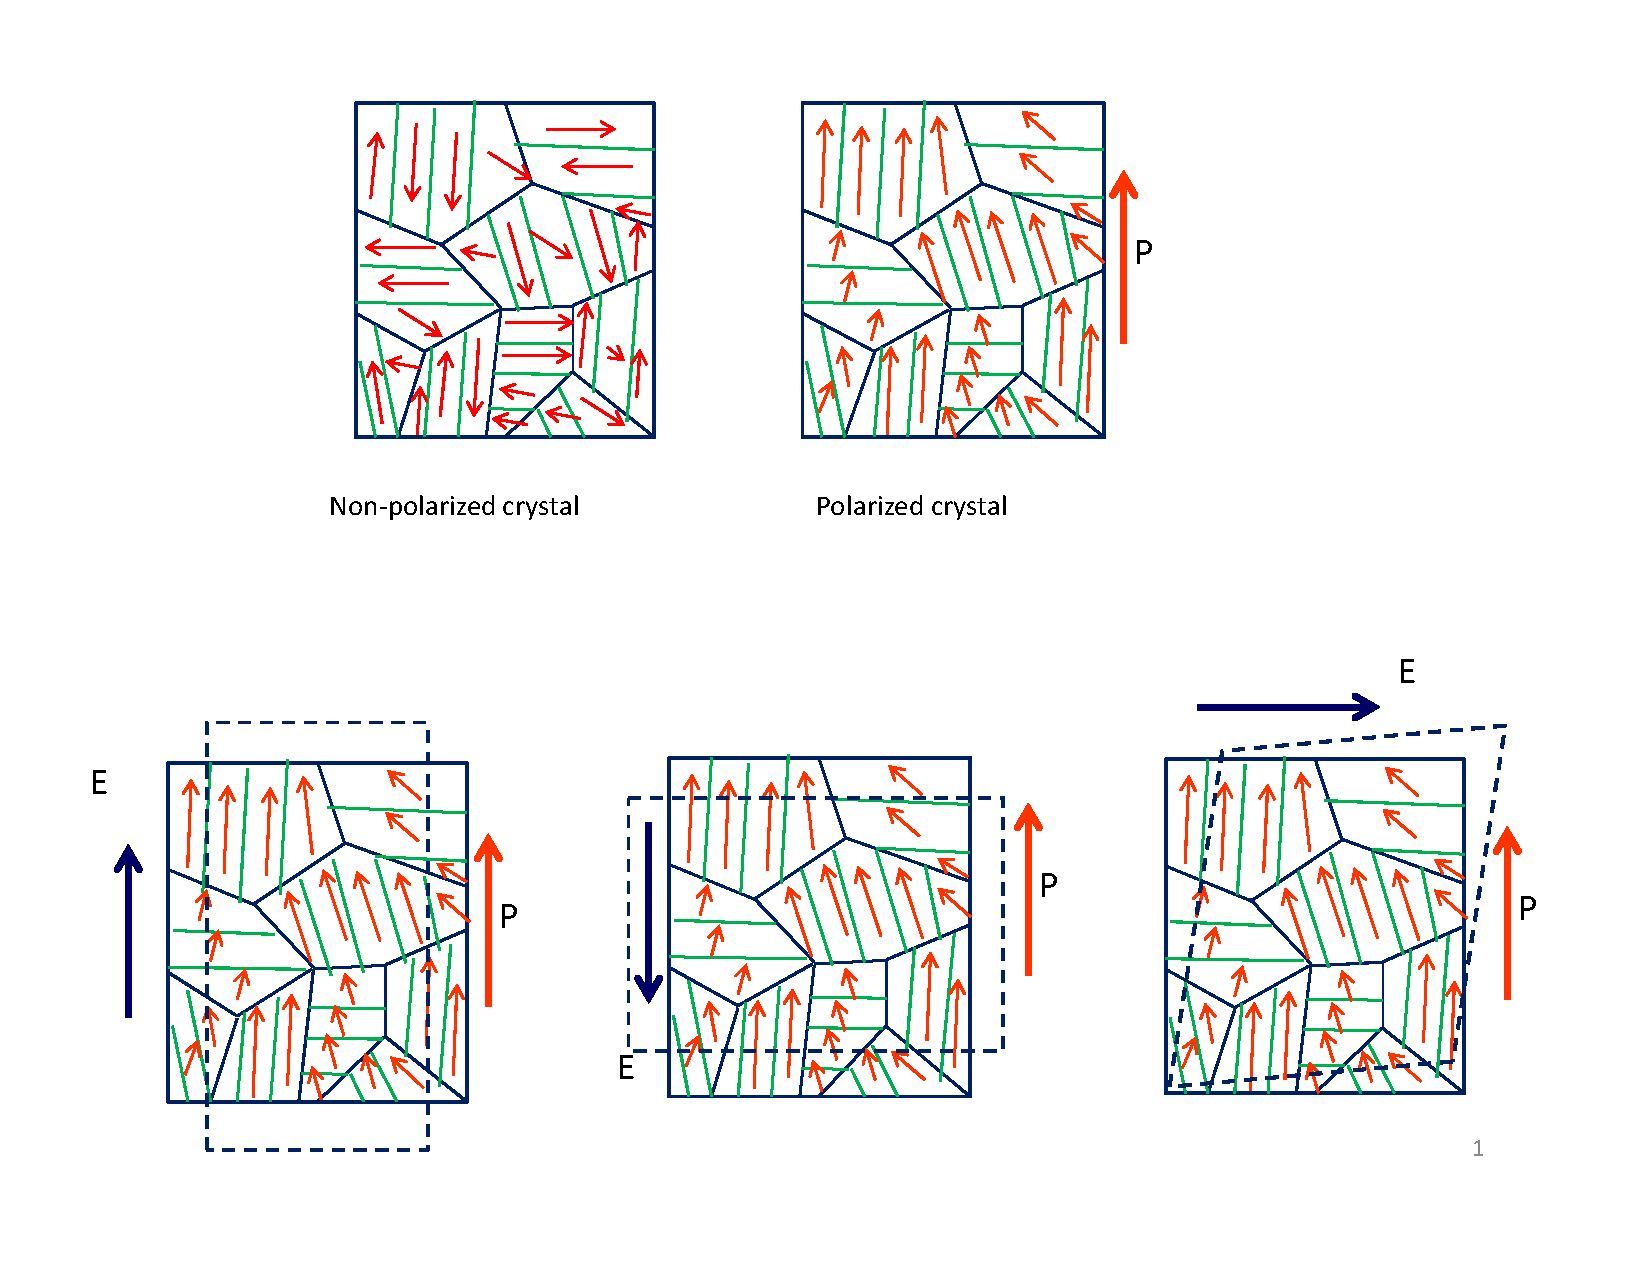
\includegraphics[height=7cm]{../images/grain_polarization_piezo_electric.pdf}\\ 
\end{frame}

\begin{frame}{Typical behavior of bulk PZT under cyclic electric field} 

\centering
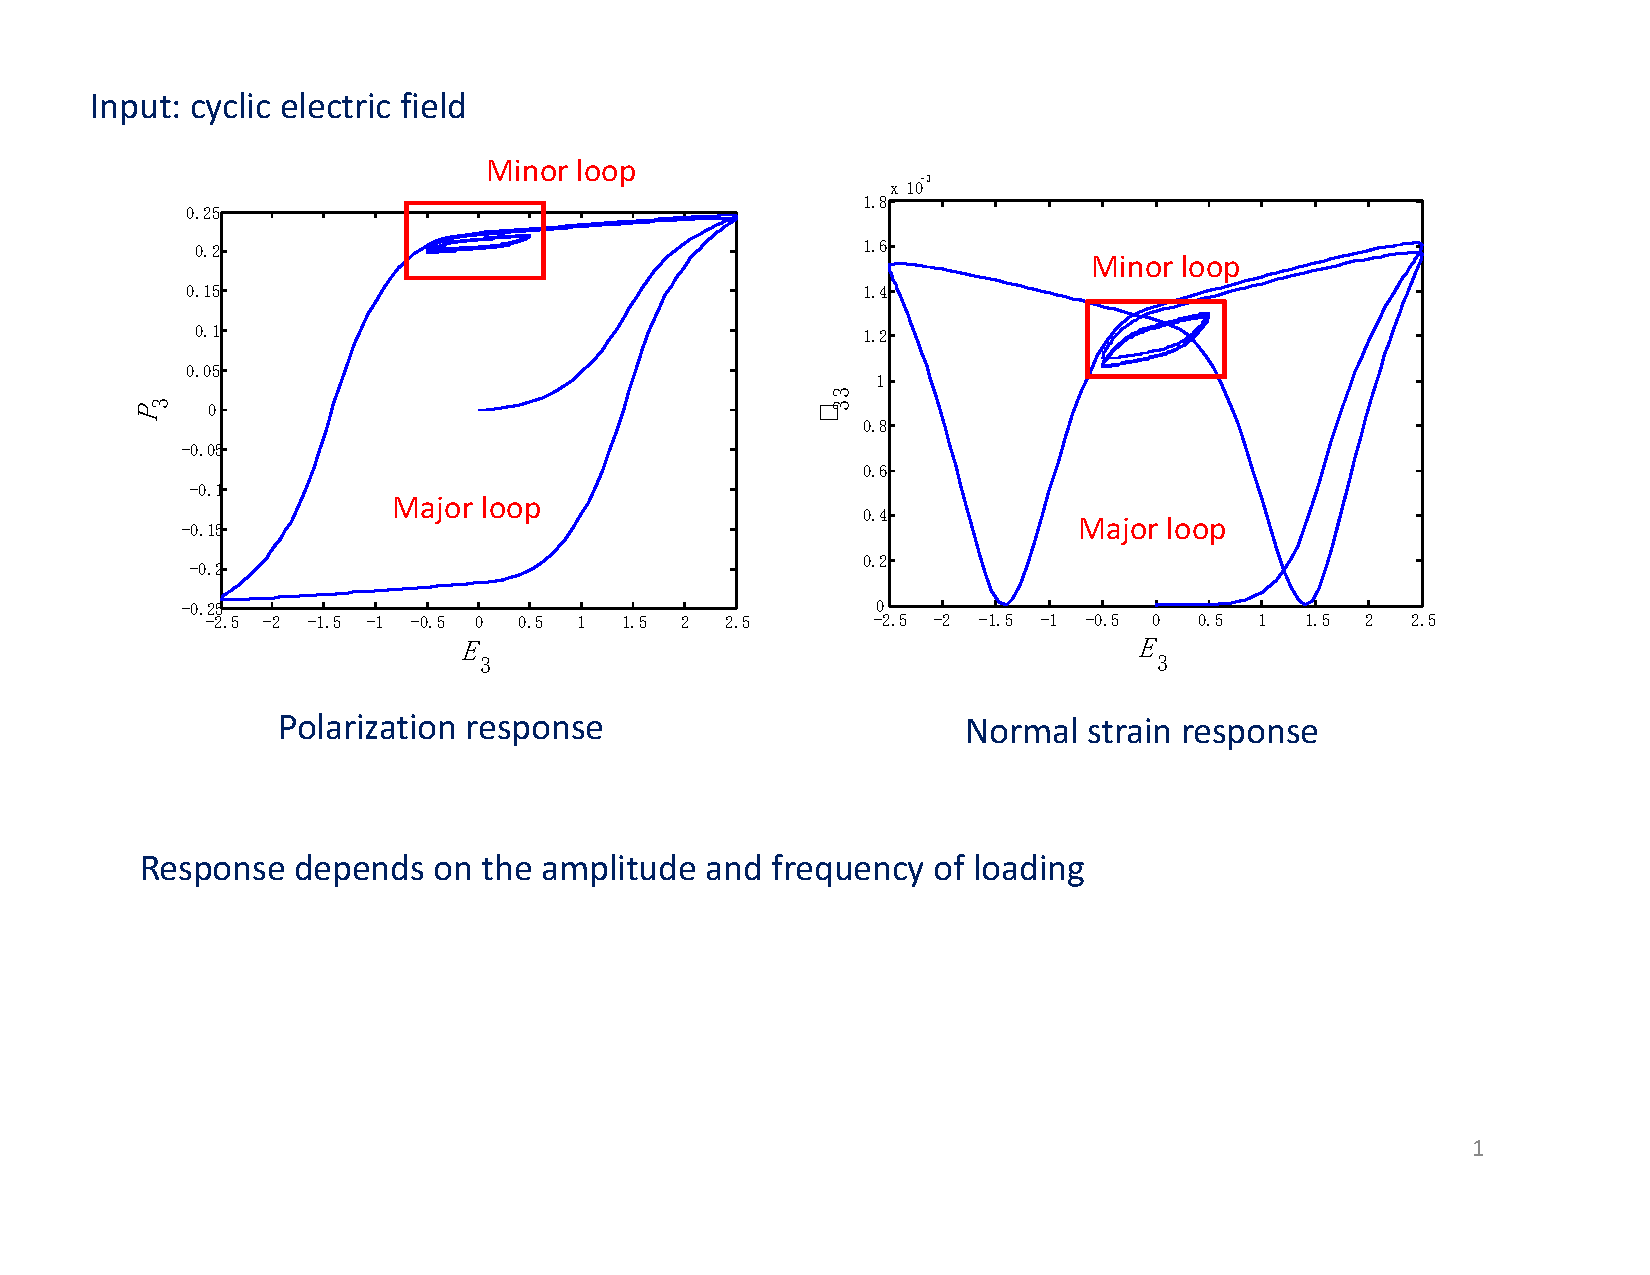
\includegraphics[height=7cm]{../images/polariztion_and_stress_response.pdf}\\ 
\end{frame}

\subsection{Electromechanical Response} 

\begin{frame}{Constitutive Equation} 

The relationship between stress $\sigma_{11}$ and
strain $\varepsilon_{11}$, and electric field $E_3$ and electric flux $D_3$.
\begin{block}<+->{Electromechanical Constitutive Equation}
\begin{equation}
\begin{aligned}
&\sigma_{11}=C_{1111} \varepsilon_{11}-e_{311} E_{3} \\
&D_3=e_{311} \varepsilon_{11}+\kappa_{33}^\varepsilon E_{3}
\end{aligned}
\label{stress_1D_const_eqn_beam:EQN}
\end{equation}
\end{block}

$C_{1111}$ is the elastic stiffness. \\
$e_{311}$ is the piezoelectric constant. \\
$\kappa_{33}^\varepsilon$ is the permittivity at constant strain. \\

\end{frame}


\begin{frame}{Constitutive Equation} 

Extending the constitutiv equation to 3D
\begin{block}<+->{Electromechanical Constitutive Equation}
\begin{equation}
\begin{aligned}
&\sigma _{ij} = 
\sum_{k,l=1}^3 {C_{ijkl}}{\varepsilon _{kl}} - 
\sum_{k=1}^3 {e_{kij}}{E_k}\\
&{D_k} = 
\sum_{i,j=1}^3 e_{kij}\varepsilon _{ij} + 
\sum_{j=1}^3 \kappa _{kj}{E_j}\\
& (i,j,k=1 \dots 3)
\end{aligned}
\label{EQN:Standanrd_Constitutive_Relation} 
\end{equation}
\end{block}
This is the standard constitutive equation presented in IEEE standard
\cite{meitzler1988ieee}.
\end{frame}


\begin{frame}{The Non Linear and time Dependent Responce}
Nonlinear and hysteretic response of piezoelectric structures under cyclic
electric field input

\begin{columns}[t]
     \begin{column}[T]{5cm}
     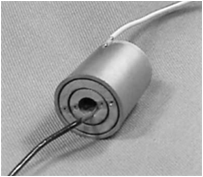
\includegraphics[height=4cm]{../images/telescpic_actuator_picture}\\ 
Telescopic Actuator \cite{Berner1999} 
     \end{column}
     \begin{column}[T]{5cm} % alternative top-align that's better for graphics    
      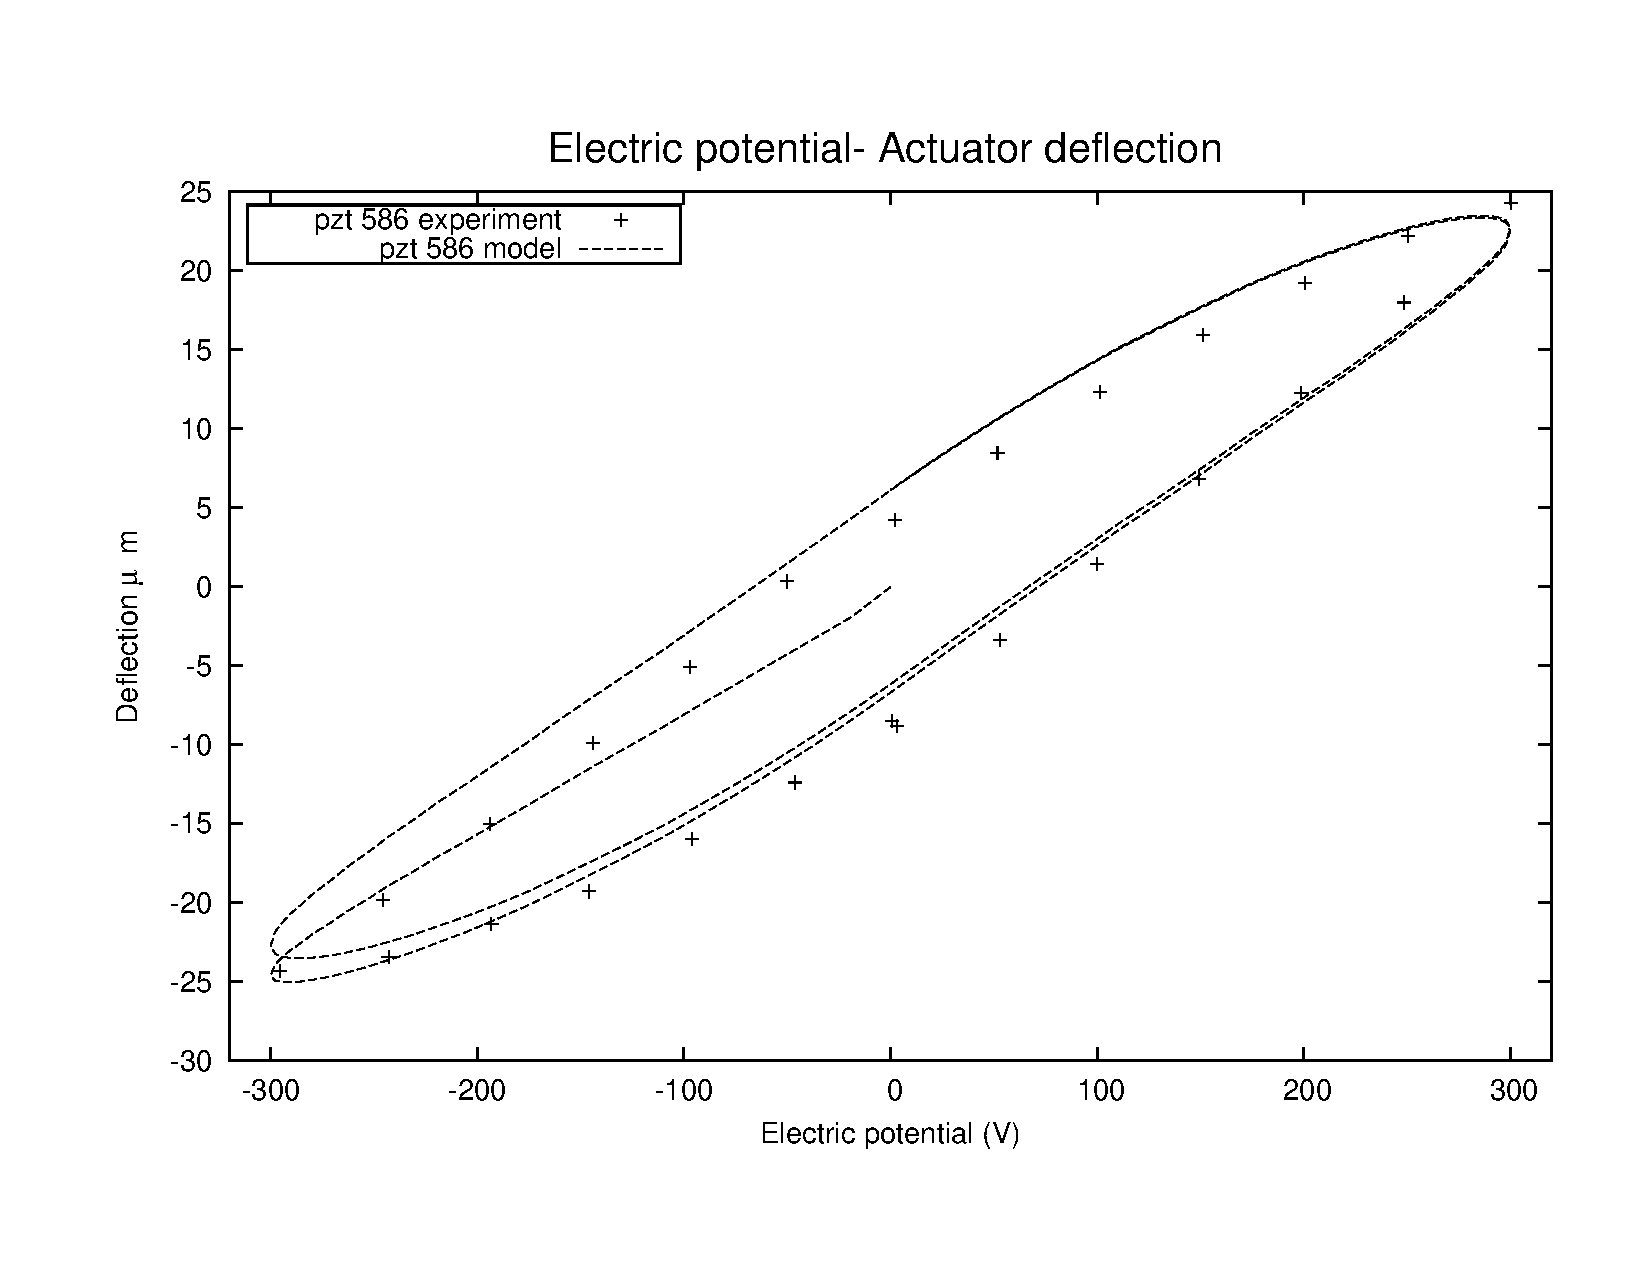
\includegraphics[height=4cm]{../images/result_pzt_586.pdf}\\
      Deflection Response
     \end{column}
     \end{columns}    
\end{frame}

\subsection{Motivation}

\begin{frame}{Research Motivations}
\begin{itemize}\itemsep2ex

\item	Formulate nonlinear time-dependent electromechanical constitutive models
of piezoelectric materials
\item	Develop finite element model for analyzing structures with proposed
constitutive equation

\end{itemize}     
\end{frame}
 
\section{Electromechanical Constitutive Models}

\subsection{Non Linear Time Dependent Model for Polarized State}

\begin{frame}{Linear time dependent Electromechanical model}
  \begin{itemize}
  \item  Constitutive relation with normalized time functions
\end{itemize} 
\fontsize{8pt}{8pt}

\begin{block}<+->{Nonlinear and time dependent constitutive equation}
\begin{equation}
\begin{aligned}
&\sigma_{ij}(t)=\int_{0^-}^t \sum_{k=1}^{3} \sum_{l=1}^{3} K^C_{ijkl}(t-s) \frac{\partial \sigma_{ij}(s)}{\partial \varepsilon_{kl}(s)}\dot{\varepsilon}_{kl}(s)ds +\int_{0^-}^t \sum_{k=1}^{3} K^e_{kij}(t-s) \frac{\partial \sigma_{ij}(s)}{\partial E_{k}(s)} \dot{E}_{k} (s)ds 
\\
&D_k(t)=\int_{0^-}^t \sum_{i=1}^{3} \sum_{j=1}^{3} K_{kij}^e(t-s) \frac{\partial D_{k}(s)}{\partial \varepsilon_{ij}(s)}\dot{\varepsilon}_{ij}(s)ds +\int_{0^-}^t \sum_{i=1}^{3} K_{ki}^{\kappa}(t-s) \frac{\partial D_{k}(s)}{\partial E_{i}(s)} \dot{E}_{i} (s)ds 
\end{aligned}
\label{EQN:NormalizedConstitutiveRelation}
\end{equation}  
\end{block}
\end{frame}

\begin{frame}{Material Field Variables}

\begin{block}<+->{Derivatives of the linear field variables}
\begin{equation}
\begin{aligned}
&\frac{\partial \sigma_{ij}(s)}{\partial \varepsilon_{kl}(s)}=C_{ijkl} \\
&\frac{\partial \sigma_{ij}(s)}{\partial E_{k}(s)}=-e_{kij} \\
&\frac{\partial D_{k}(s)}{\partial E_{i}(s)}=\kappa_{ki}
\end{aligned}
\label{EQN:Linear_Constants}
\end{equation}  
\end{block}

\end{frame}

\begin{frame}{Kernel Functions}
\begin{block}<+->{Series of exponential functions, often called Prony series, is used for kernel function}
\begin{equation}
\label{EQN:LrgKProney}
\begin{aligned}
&K_{ijkl}^C(t) =\sum_{I=0}^{NP}{}^{I}K_{ijkl}^{C} exp(-{}^{I}\lambda_{ijkl}^{C}t) \\
&K_{ijk}^e(t) =\sum_{I=0}^{NP}{}^{I}K_{ijk}^{e} exp(-{}^{I}\lambda_{ijk}^{e}t) \\
&K_{ki}^\kappa(t) =\sum_{I=0}^{NP}{}^{I}K_{ki}^{\kappa} exp(-{}^{I}\lambda_{ki}^{\kappa}t) \\
\end{aligned}
\end{equation}
\end{block} 
\end{frame}

\begin{frame}{Constitutive Equation}
It is possible to use a developed nonlinear static constitutive equation in the
time dependent framework.
\begin{block}<+->{Time Independent Non Linear Constitutive Equation \cite{Tiersten1993}}
\begin{equation}
\begin{aligned}
&\sigma_{ij}=C_{ijkl}\varepsilon_{kl}-e_{kij}E_k-\frac{1}{2}\widehat{b}_{klij}E_k E_l
\\
&D_k=e_{kij}\varepsilon_{ij}+\kappa_{ki}E_i+\frac{1}{2}\chi_{kij}E_i E_j
\end{aligned}
\label{EQN:NonLinearElectroMechancialConstants}
\end{equation}
\end{block} 
\end{frame}

\begin{frame}{Material Field Variables}
Using the nonlinear electromechanical coupling constitutive equation.
\begin{block}<+->{Derivatives of the field variables}
\begin{equation}
\begin{aligned}
&\frac{\partial \sigma_{ij}(s)}{\partial \varepsilon_{kl}(s)}=C_{ijkl} \\
&\frac{\partial \sigma_{ij}(s)}{\partial E_{k}(s)}=-e_{kij}-\widehat{b}_{klij} E_l\\
&\frac{\partial D_{k}(s)}{\partial E_{i}(s)}=\kappa_{ki}+\chi_{kij} E_j\\
&\frac{\partial D_{k}(s)}{\partial \varepsilon_{kl}(s)}=e_{kij}
\end{aligned}
\label{EQN:Non_LinearLinear_Constants}
\end{equation}
\end{block} 

\end{frame}

\subsection{Polarization Switching}

\begin{frame}{On polarization switching}
     \begin{columns}[t]
     \begin{column}[T]{5cm}
       \begin{itemize} \itemsep15ex
  \item  Minor Loop 
  
  \item  Major Loop
  \end{itemize} 
     \end{column}
     \begin{column}[T]{10cm} % alternative top-align that's better for graphics          
      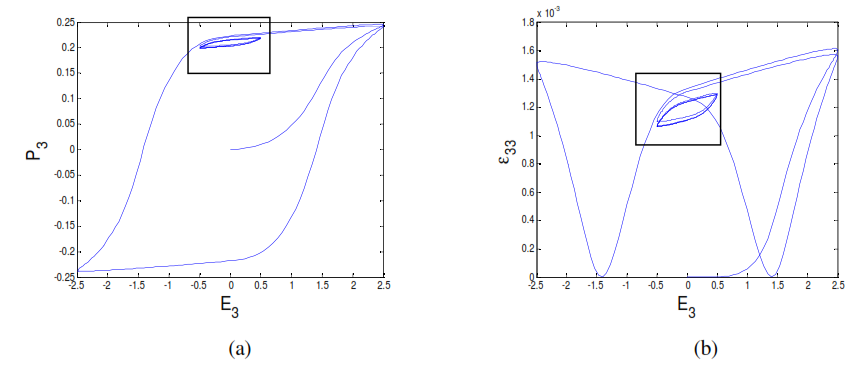
\includegraphics[height=3cm]{../images/Miror_Loop_Hystersis_Response}\\
       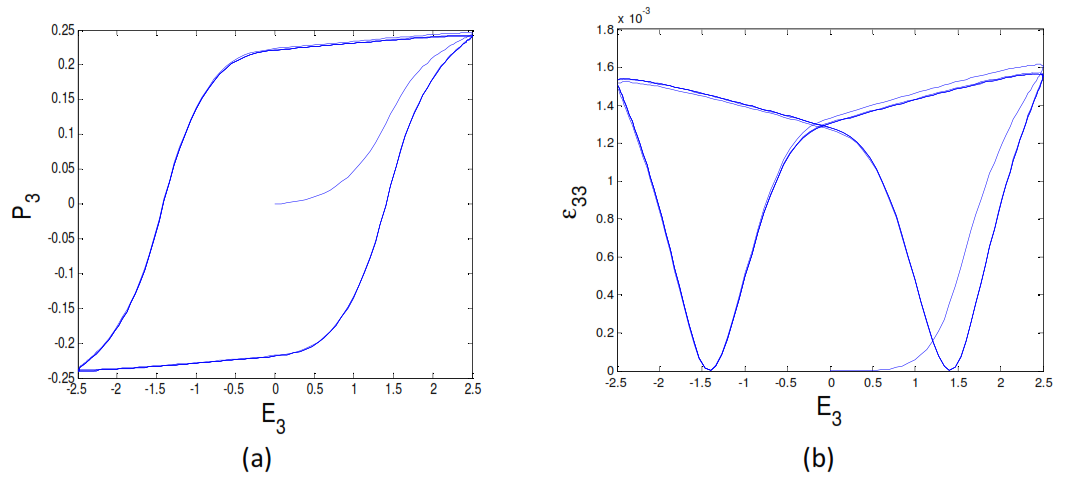
\includegraphics[height=3cm]{../images/Major_Loop_Hystersis_Response}\\
     \end{column}
     \end{columns}    
\end{frame}

\begin{frame}{Additive Decomposition of Polarization}
Consider an electric field input in the $x_3$ direction $E_3(s)$, and $E_3(s)=0,\forall s<0$  , where $s$ is the time history.  The corresponding polarization response at the current time $t$ is:
\begin{block}<+->{Additive decomposition of Polarization}
\begin{equation}
P_3^t\equiv P_3[E_3(t-s),t]=R[E_3(t-s),t]+Q[E_3(t-s),t]
\label{EQN:PolRQ}
\end{equation}
\end{block} 
\end{frame}


\begin{frame}{Time Dependent Reversible Polarization}
\fontsize{9pt}{9pt}

\begin{block}<+->{The reversible polarization response is expressed as:}
\begin{equation}
\label{EQN:RevPol}
R^t\equiv R[E_3(t-s),t]= R[E_3^0,t]+\int_{0^+}^t\frac{\partial R}{\partial E_3} [E_3^t,t-s] \frac{dE_3^s}{ds}ds , t \geq 0
\end{equation}
\end{block} 

\begin{equation}
\label{EQN:StaticRevPol}
R[E_3^0,t]=R_0(E_3^0)+R_1(E_3^0)\big(1-exp\bigg[-\frac{t}{\tau_1}\bigg] \big)
\end{equation}
\begin{equation}
\label{EQN:R0R1Defini}
\begin{aligned}
&R_0(E_3^s)=\kappa_0 E_3^s \\
&R_1(E_3^s)=\kappa_1 E_3^s
\end{aligned}
\end{equation}
\end{frame}

\begin{frame}{Evolution Law for Irreversible Polarization}
  \begin{itemize}
  \item  Irreversible polarization is formed when $f(P_3^t,P_c)=0$ and $E_3^t P_3^t>0$
\end{itemize}
\fontsize{9pt}{9pt}
\begin{equation}
\label{EQN:IrrevePol}
Q^t\equiv Q[E_3^t]= \int_{0^+}^{E_3^t}\frac{d Q^s}{d E_3}{dE_3}
\end{equation}

\begin{equation}
\frac{d Q^t}{d E_3}=
  \begin{cases}
   \lambda|\frac{E_3^t}{E_c}|^n& \text{if } |E_3^t|\leq E_c, f=0 \\
\mu . exp[-\omega(\frac{|E_3^t|}{E_c}-1)] & \text{if }|E_3^t|> E_c, f=0 \\ 0
& \text{if } f\leqslant 0 \\
  \end{cases}
\label{EQN:TimeDepIrrevePol}  
\end{equation}
\begin{equation}
\label{EQN:SurfacePol}
f(P_3^t,P_c)={P_3^t}^2-P_c^2
\end{equation}
\end{frame}


\begin{frame}{Constitutive Equation Beyond Coercive Limit}
  \begin{itemize}
  \item  A nonlinear polarization switching electromechanical coupling
  constitutive model
\end{itemize}
\fontsize{9pt}{9pt}
\begin{equation}
\label{EQN:3D_Polarization_Switching}
\begin{aligned}
&  \varepsilon _{ij}^t = {S_{ijkl}}\sigma _{kl}^t + 4g_{nij}^t{\kappa _{nm}}g_{mkl}^t\sigma _{kl}^t + 2 g_{kij}^t P_k^t \hfill \\
&  D_i^t = 2{\kappa _{im}}g_{mkl}^t\sigma _{kl}^t + P_i^t \hfill \\ 
\end{aligned}
\end{equation}

\begin{equation}
\label{EQN:Trasverse_Polarization}
P_1^t = {\kappa _{11}}E_1^t\ ; P_2^t = {\kappa _{22}}E_2^t 
\end{equation}

\begin{equation}
\label{EQN:Elec_Mech_Constants_3D}
g_{ijk}^t \equiv g_{ijk} (P_3^t) = \frac{P_3^t}{P_r}{e^{ - \left| {P_3^t} \right|/C_1}}g_{ijk}^r\
\end{equation}
\end{frame}

\section{Finite Element Formulation}
\subsection{Electromechanical Finite Element Model}

\begin{frame}{The Virtual Work}

\begin{block}<+->{Variational formulation}
\begin{equation}
\delta \pi= \int_V \sigma_{ij}\delta \varepsilon_{ij} dV -\int_V D_{i}\delta E_{i} dV-\int_{\partial V} T_{i}\delta u_{i} d{\partial V}+\int_{\partial V} Q\delta \phi d{\partial V}
\label{EQN:Variation_of_Energy}
\end{equation} 
\end{block} 

The equilibrium is achived when virtual work in stationary.
\begin{equation}
R_k=\frac{\partial \delta \pi}{\partial \delta d_k}=0 ,(k=1\dots NDF)
\label{EQN:ResidualRepresentation}
\end{equation}

\end{frame}

\begin{frame}{The Finite Element Approximation}
  \begin{itemize}
  \item Degrees of freedom in each point of 3D continuum electro mechanical element
\end{itemize}

\begin{equation}
[u]^T=[u_1,u_2,u_3,\phi]^T
\label{EQN:displacement}
\end{equation}

\begin{itemize}
\item The element degrees of freedom\
\begin{equation}
[d]^T=[u_1^1,u_2^1,u_3^1,\phi^1 \dots u_1^{ND},u_2^{ND},u_3^{ND},\phi^{ND}]
\label{EQN:degreesoffreedom}
\end{equation}
\end{itemize}

\begin{itemize}
\item The approximation function\
\begin{equation}
u_i=\varphi_{ip} d_p,(i=1\dots 4),(p=1\dots NDF)
\label{EQN:DispShapeDof}
\end{equation}
\end{itemize}
\end{frame}

\begin{frame}{Defining Field Variables}
  \begin{itemize}
  \item The linear strain and electric field vector are defined as:
\end{itemize}

\begin{equation}
\begin{aligned}
&\varepsilon_{ij}=\frac{1}{2}(u_{i,j}+u_{j,i})
&E_{i}=-\phi_{,i}
\end{aligned}
\label{EQN:Linearstrain_Electri}
\end{equation}

\begin{itemize}
\item Variation of field functions\
\begin{equation}
\delta u_i=\varphi_{ip} \delta d_p,(i=1\dots 4),(p=1\dots NDF)
\label{EQN:VarDispShapeDof}
\end{equation}
\end{itemize}

\begin{itemize}
\item The tangent matrix is defined as:\
\begin{equation}
\mathcal{K}_{kl} =\frac{\partial R_k}{\partial d_l}=\frac{\partial}{\partial d_l} \frac{\partial \delta \pi}{\partial \delta d_k} ; (l,k=1\dots NDF)
\label{EQN:TangentRepresentation}
\end{equation}
\end{itemize}
\end{frame}


\begin{frame}{Explicit Expression for Residual and Tangent}
  \begin{itemize}
  \item Explicit form for residual vector:
\end{itemize}

\begin{equation}
\fontsize{7pt}{7pt}
R_k=\int_V \sigma_{ij} \frac{\partial \delta \varepsilon_{ij}}{\partial \delta d_k}  dV-\int_S T_{i} \frac{\delta u_{i}}{\partial \delta d_k}  ds-\int_V D_i \frac{\delta E_{i}}{\partial \delta d_k} dV+\int_S Q \frac{\partial \phi}{\partial \delta d_k}ds ,(k=1\dots NDF)
\label{EQN:ExplicitResidualRepresentation}
\end{equation}

\begin{itemize}
\item The tangent matrix is defined with respect to field derivatives:

\begin{equation}
\fontsize{8pt}{8pt}
\mathcal{K}_{kl} =\frac{\partial R_k}{\partial d_l}=\frac{\partial R_k}{\partial \varepsilon_{ij}}\frac{\partial \varepsilon_{ij}}{\partial d_l}+\frac{\partial R_k}{\partial E_{i}}\frac{\partial E_{i}}{\partial d_l}
\label{EQN:ExplcitTangentRepresentation}
\end{equation}
\end{itemize}

\begin{itemize}
\item The tangent matrix is explicitly defined as:
\begin{equation}
\fontsize{6pt}{6pt}
\begin{aligned}
&\frac{\partial R_k}{\partial \varepsilon_{ij}}=\int_V  \frac{\partial \sigma_{mn}}{\partial \varepsilon_{ij}} \frac{\partial \delta \varepsilon_{mn}}{\partial \delta d_k}  dV-\int_V \frac{\partial D_{p}}{\partial \varepsilon_{ij}}  \frac{\delta E_{p}}{\partial \delta d_k} dV  ,(k=1\dots NDF)\\
&\frac{\partial R_k}{\partial E_{i}}=\int_V  \frac{\partial \sigma_{mn}}{\partial E_{i}} \frac{\partial \delta \varepsilon_{mn}}{\partial \delta d_k}  dV-\int_V \frac{\partial D_{p}}{\partial E_{i}}  \frac{\delta E_{p}}{\partial \delta d_k} dV  ,(k=1\dots NDF)
\end{aligned}
\label{EQN:StressExplcitTangent}
\end{equation}
\end{itemize}
\end{frame}

\section{Result and Discussion}
\subsection{Response of Polarized Materials}

\begin{frame}{Nonlinear electromechanical coupling response}
\begin{itemize} \itemsep15ex
\item The static nonlinear response of PZT-5A results compared with experiments \cite{Crawley1990}
  \end{itemize} 
  
\begin{figure}
\centering
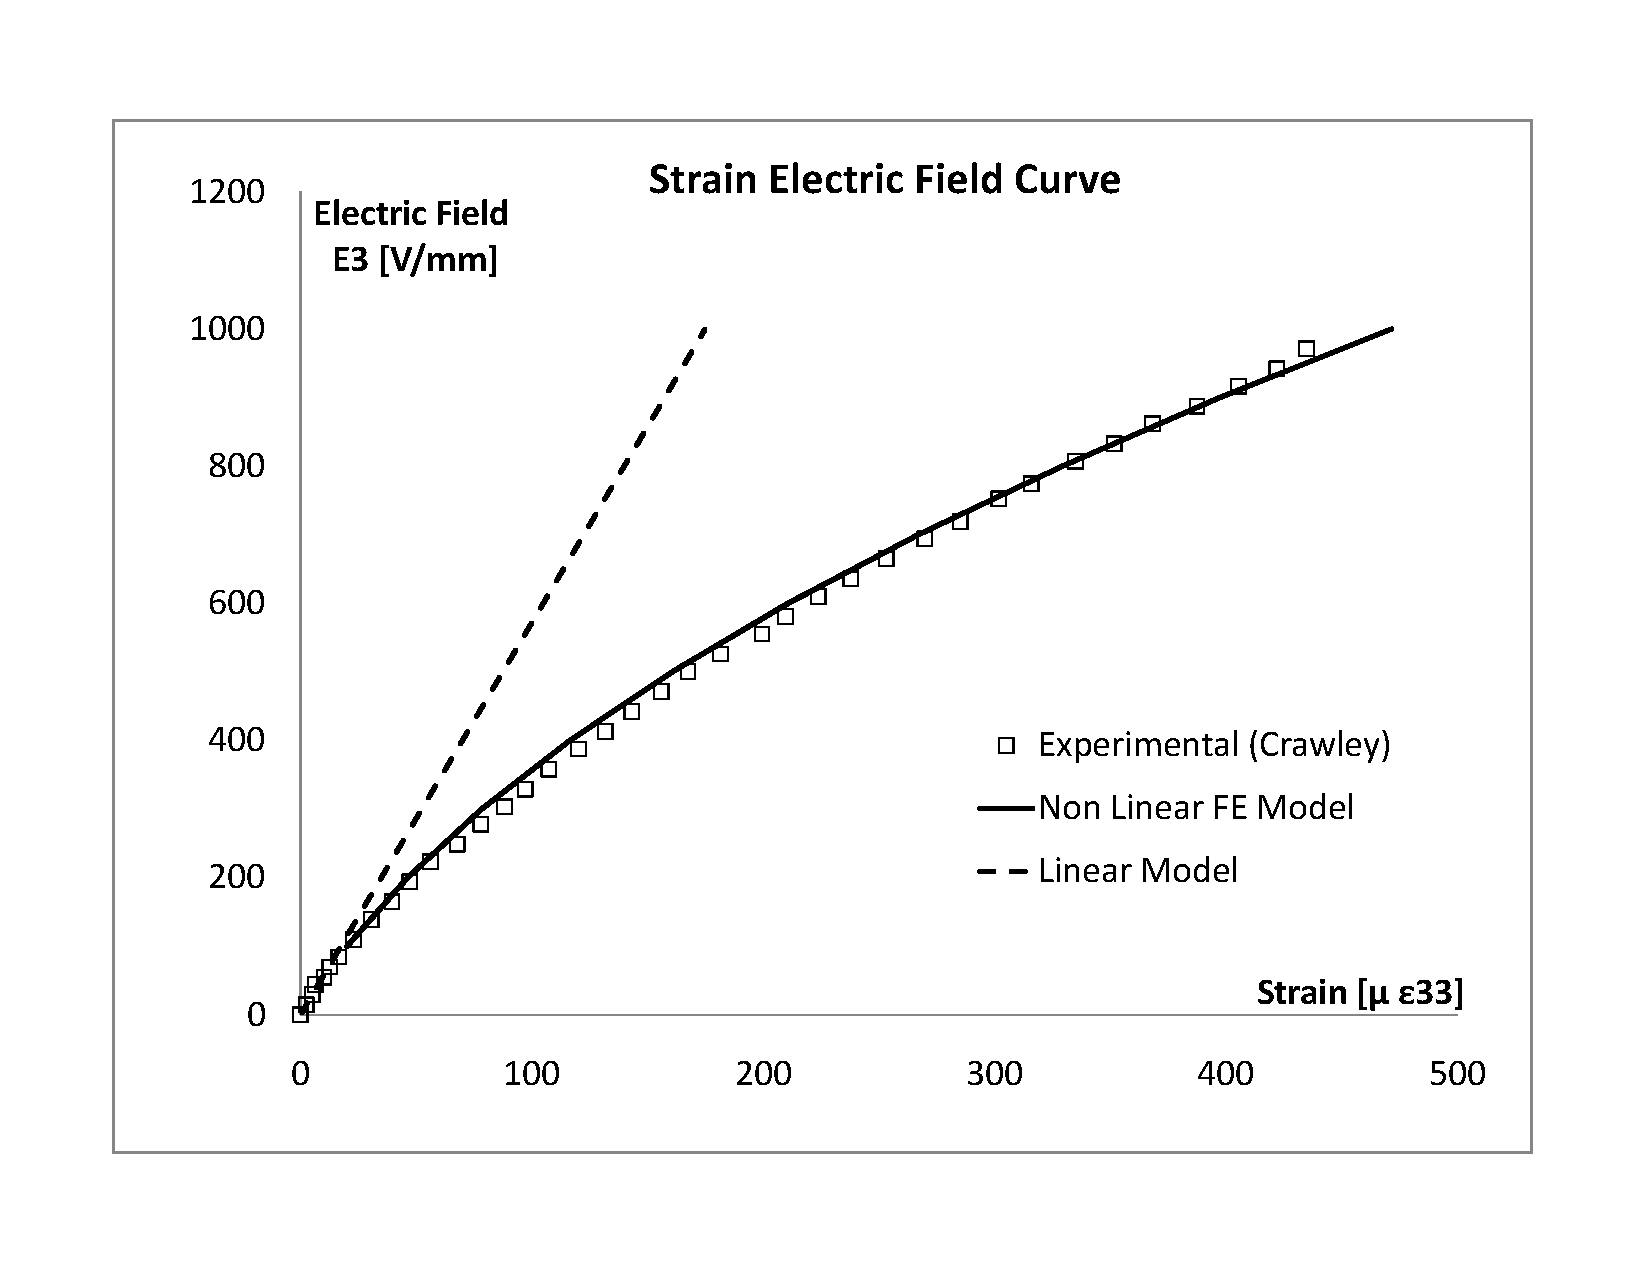
\includegraphics[height=6cm]{../images/Static_PZT_5A_FEM_Linear_XP.pdf}
\label{fig:StatilNonLinCrawley}
\end{figure}
\end{frame}


\begin{frame}{Nonlinear electromechanical coupling response}
 \begin{itemize} 
 \item Nonlinear time dependent strain response under electric field 0.1 [Hz] compared with experiment \cite{Crawley1990}
\end{itemize} 
  
\begin{figure}
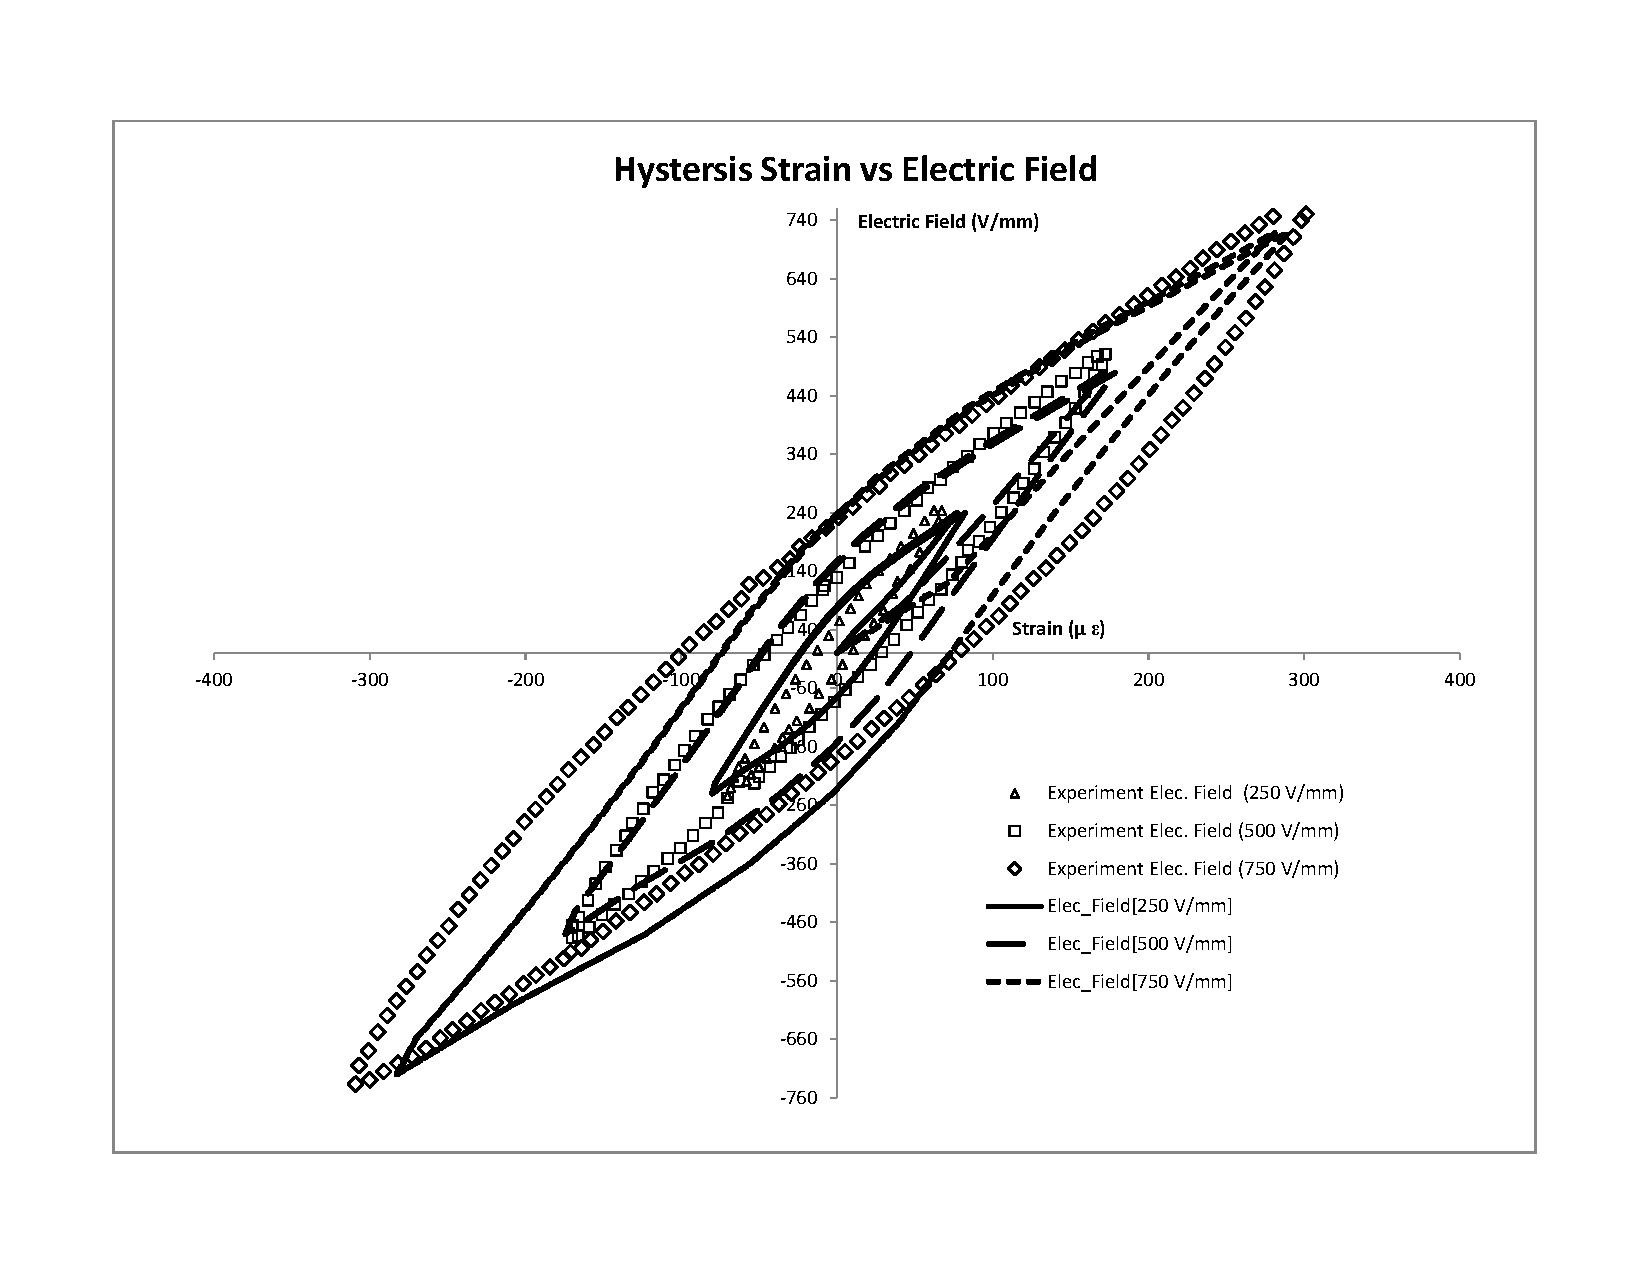
\includegraphics[height=5cm]{../images/NonLinear_Time_Dependent_Strain_Response.pdf}
\label{fig:TimeDepenNonLinCrawley}
\end{figure}

\end{frame}


\subsection{Polarization Switching Response}

\begin{frame}{Nonlinear electromechanical coupling response}
   \begin{itemize}
  \item Hysteresis polarization (a) and butterfly strain (b) responses for PZT51 at zero stress compared with experiment \cite{raey}
  \end{itemize} 
\begin{figure}
\centering
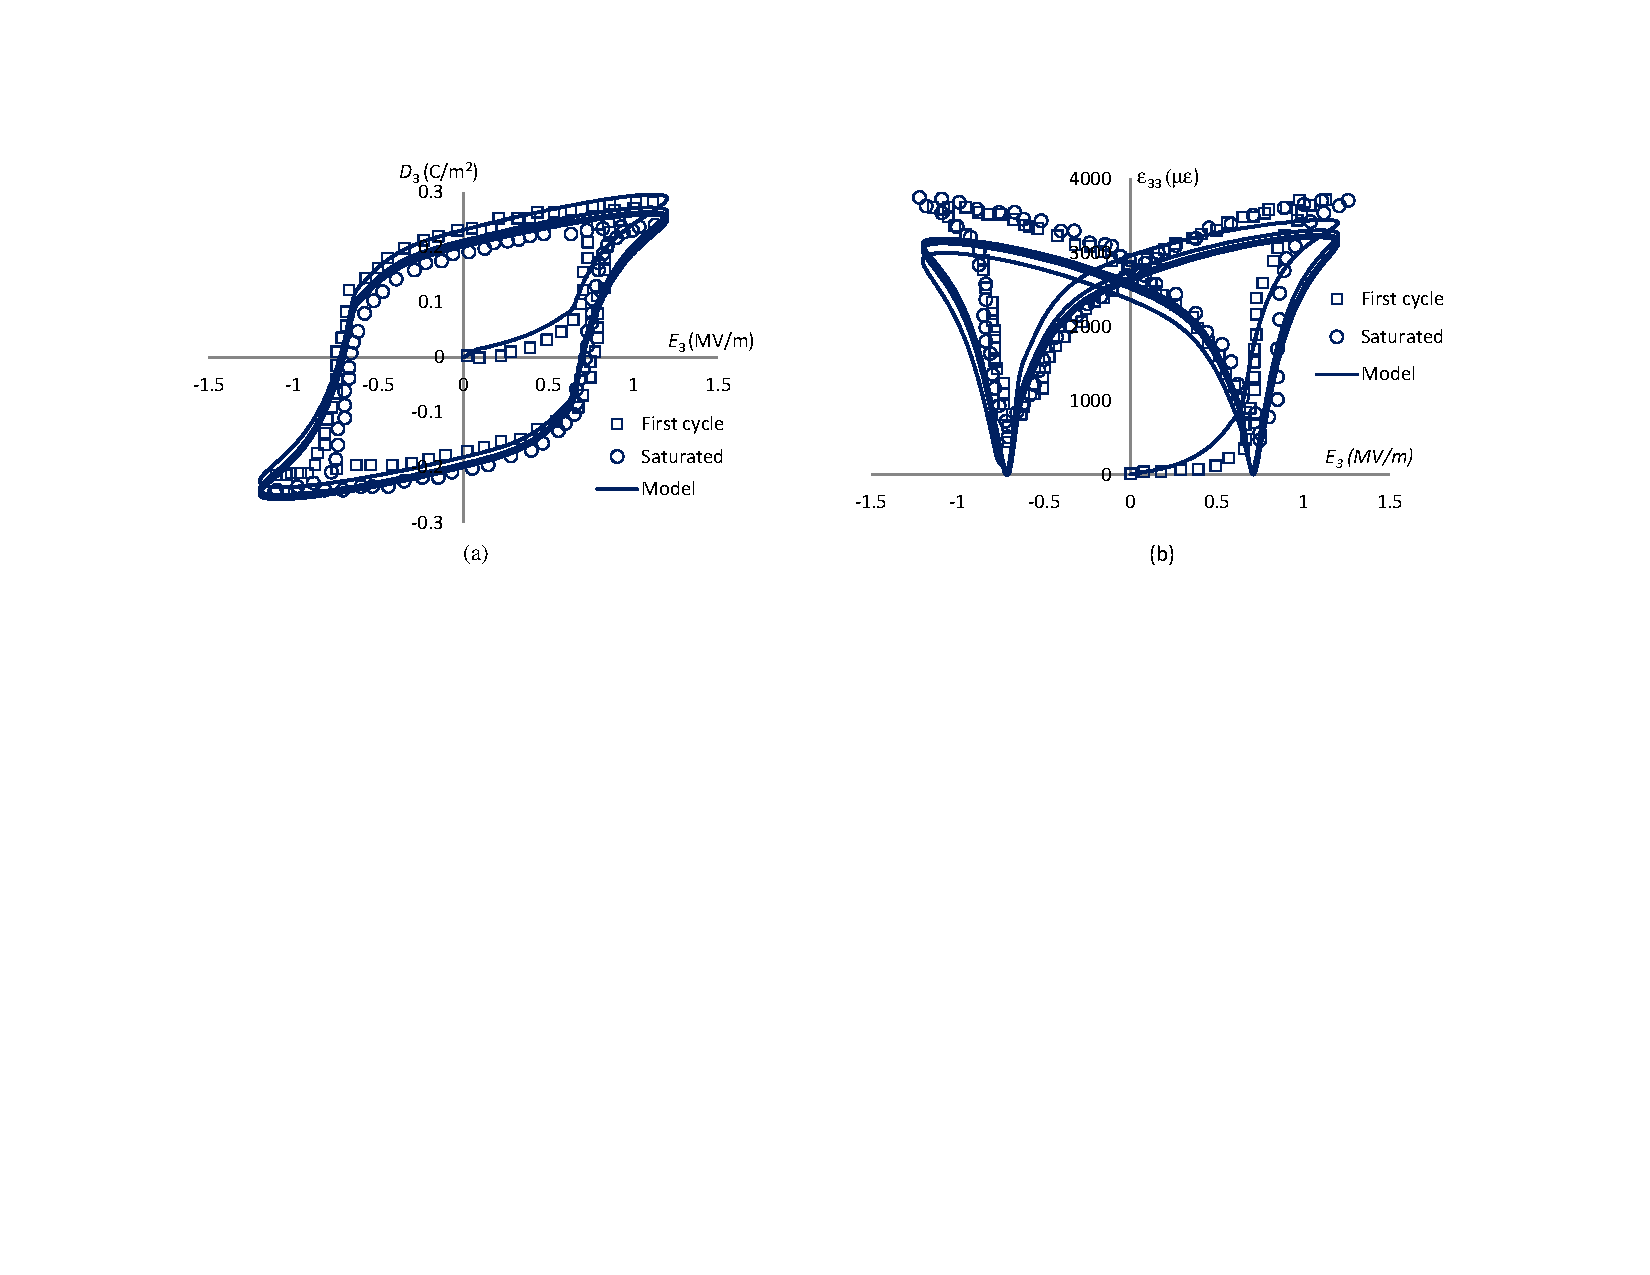
\includegraphics[scale=0.55,trim = 30mm 100mm 50mm 30mm]{../images/HysteresisPolarizationButterflyStrainResponsesPZT51ZeroStress.pdf}
\end{figure}
\end{frame}


\begin{frame}{Nonlinear electromechanical coupling response}
\fontsize{6pt}{6pt}
   \begin{itemize}
  \item Butterfly strain responses under constant compressive stresses for PZT51 compared with experiment \cite{raey}
  \end{itemize} 
  
\begin{figure}
\centering
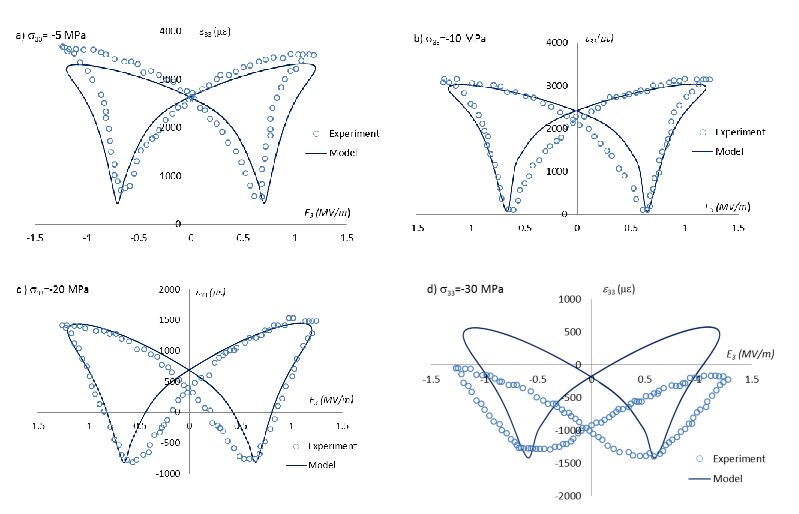
\includegraphics[height=6.5cm]{../images/ButterflyStrainResponsesUnderConstantCompressiveStresses}

\label{fig:ButterStressPolSwitchingStrainZeroStressPZT51}
\end{figure}
\end{frame}


\subsection{Structural Analyses}

\begin{frame}{Telescopic Actuator Geometry}
     \begin{columns}[t] % contents are top vertically aligned
     \begin{column}[T]{3cm} % each column can also be its own environment
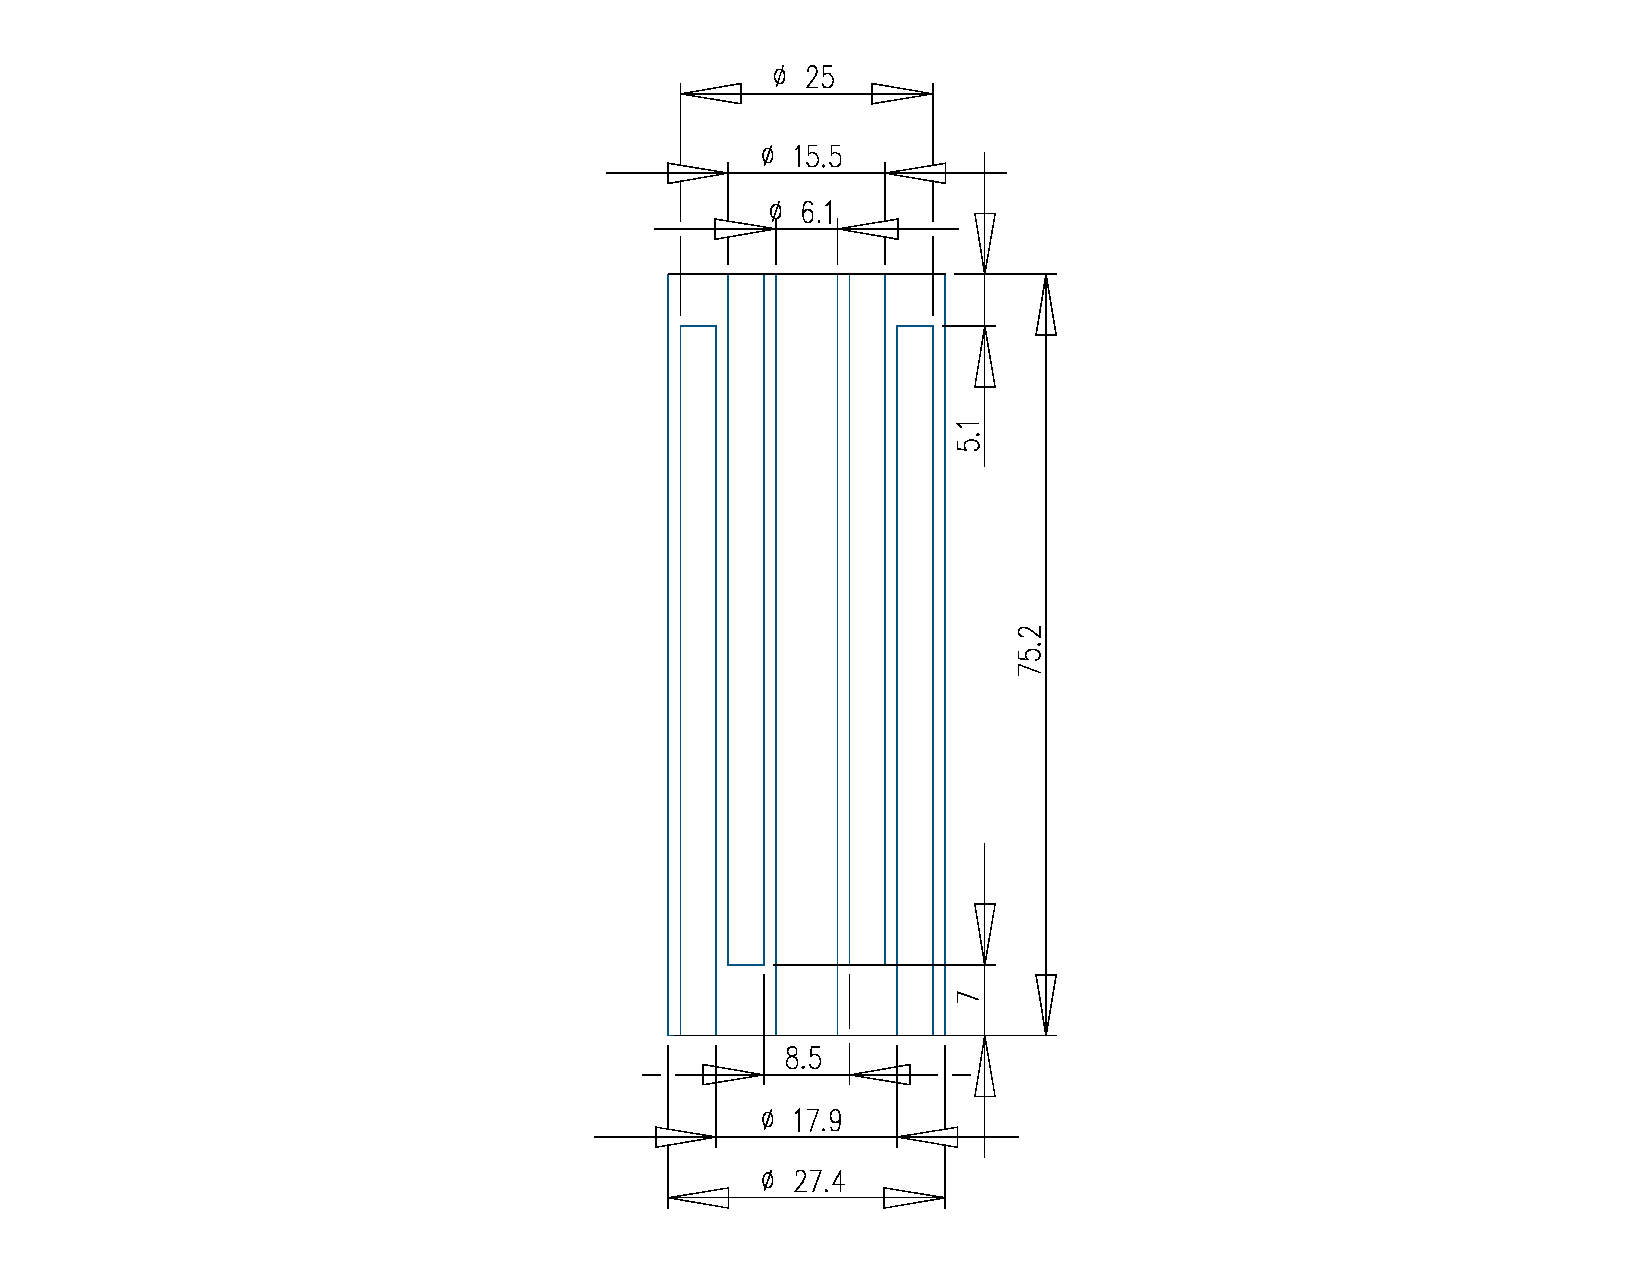
\includegraphics[trim={8cm 0 0cm 0},clip,height=3cm]{../images/PZT_586_Geometry.pdf}\\  
Geometry
     \end{column}
     \begin{column}[T]{3cm}  
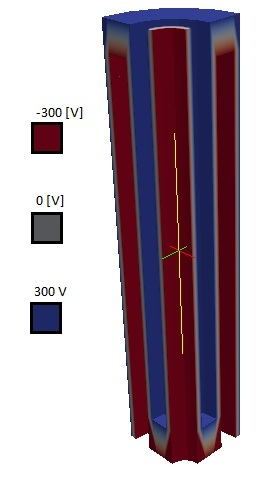
\includegraphics[height=3cm]{../images/PZT_586_Epot_Distribution}\\
Electric Potential
     \end{column}
     \begin{column}[T]{4cm}  
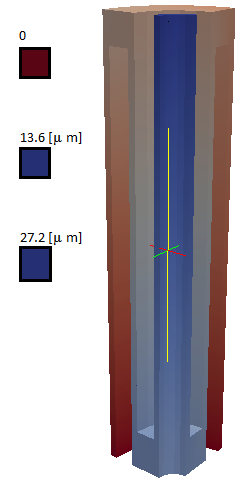
\includegraphics[height=3cm]{../images/PZT_586_Axial_Deformation}\\
Axial Deformation
     \end{column}
          
     \end{columns}    
\end{frame}

\begin{frame}{Patched Beam} 
\begin{figure}
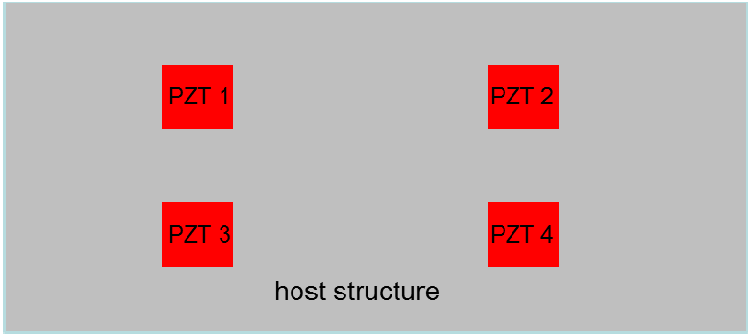
\includegraphics[height=4cm]{../images/Patched_Beam_Geometry}\\
\caption{Geometry of plate with PZT patches}
\end{figure}
\end{frame}


\begin{frame}{Tip Deflection of Patched Beam} 
\begin{figure}
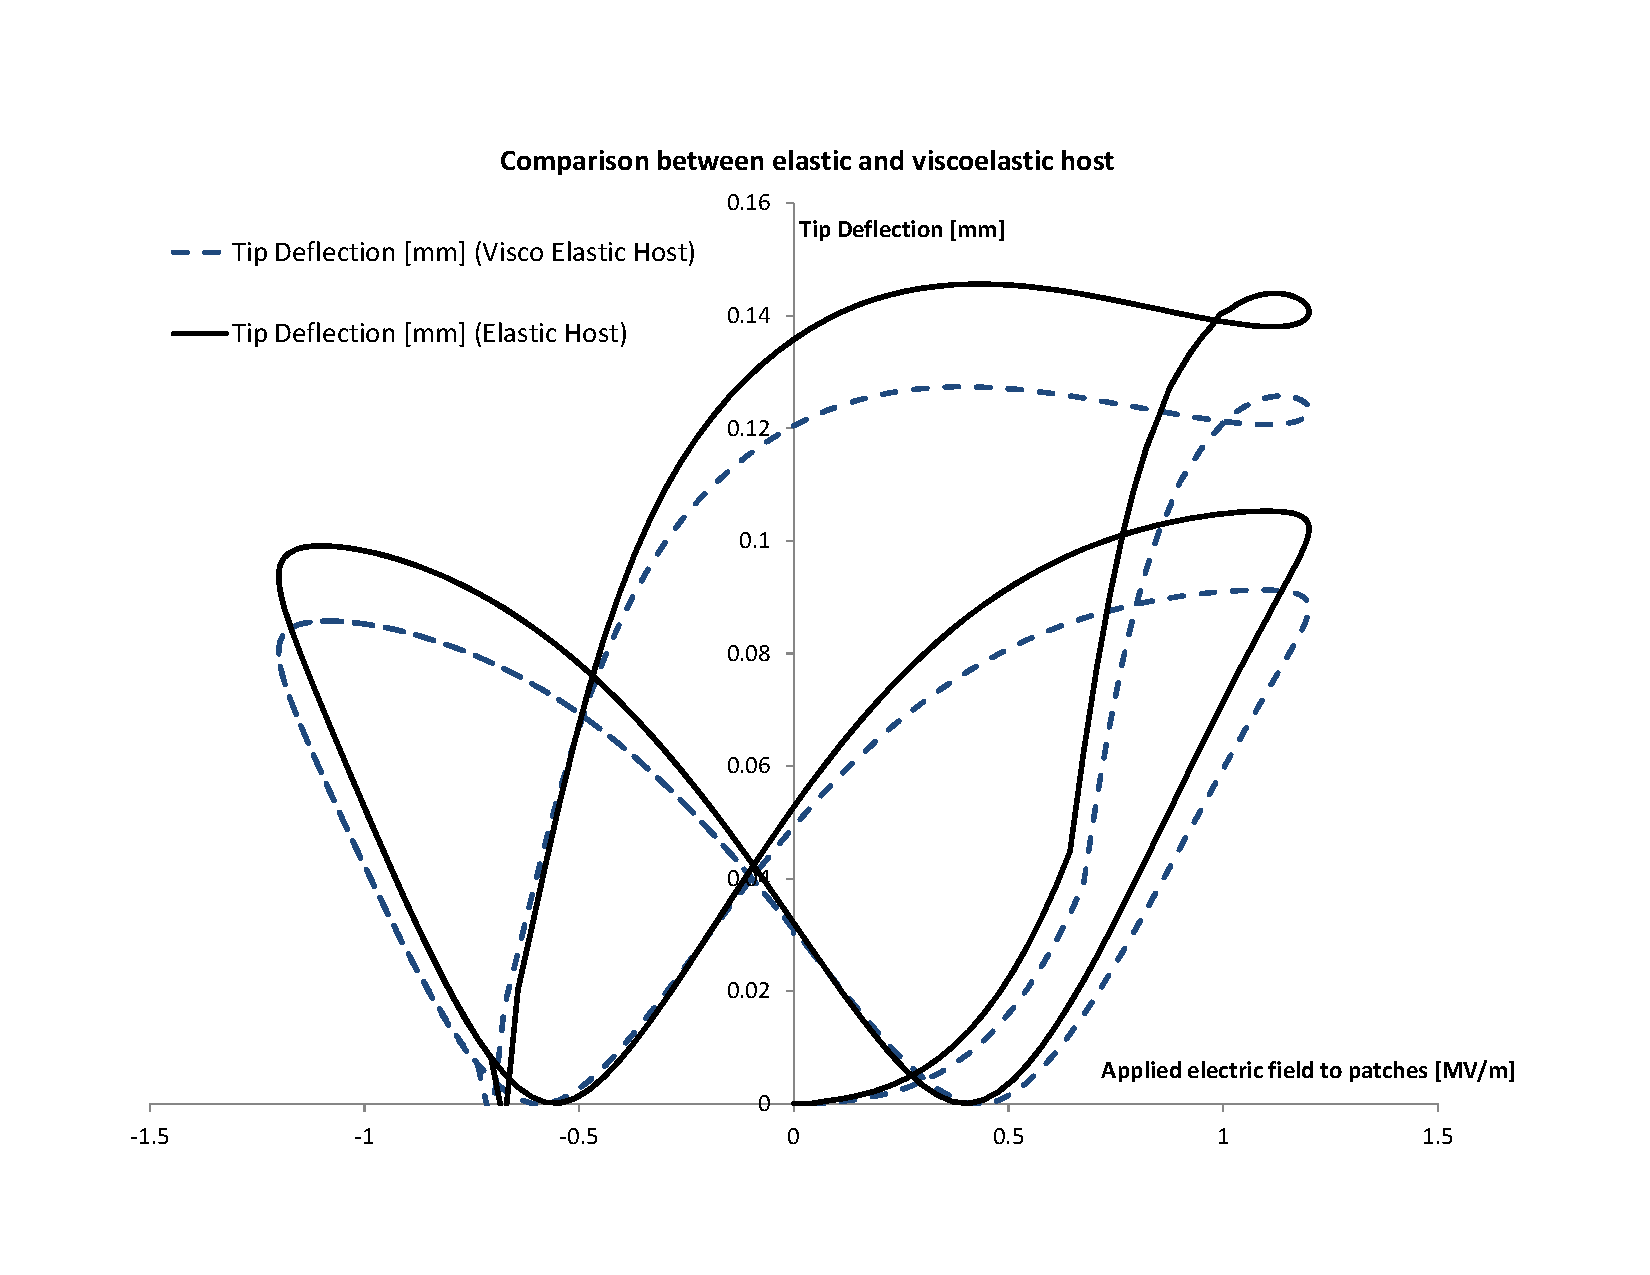
\includegraphics[height=5cm]{../images/ViscoHostCompositeActiveBeam}
\caption{Tip deflection of uniform cyclic electric fields applied patches}
\end{figure}
\end{frame}

\begin{frame}{Tip Deflection of Patched Beam}
\begin{figure}
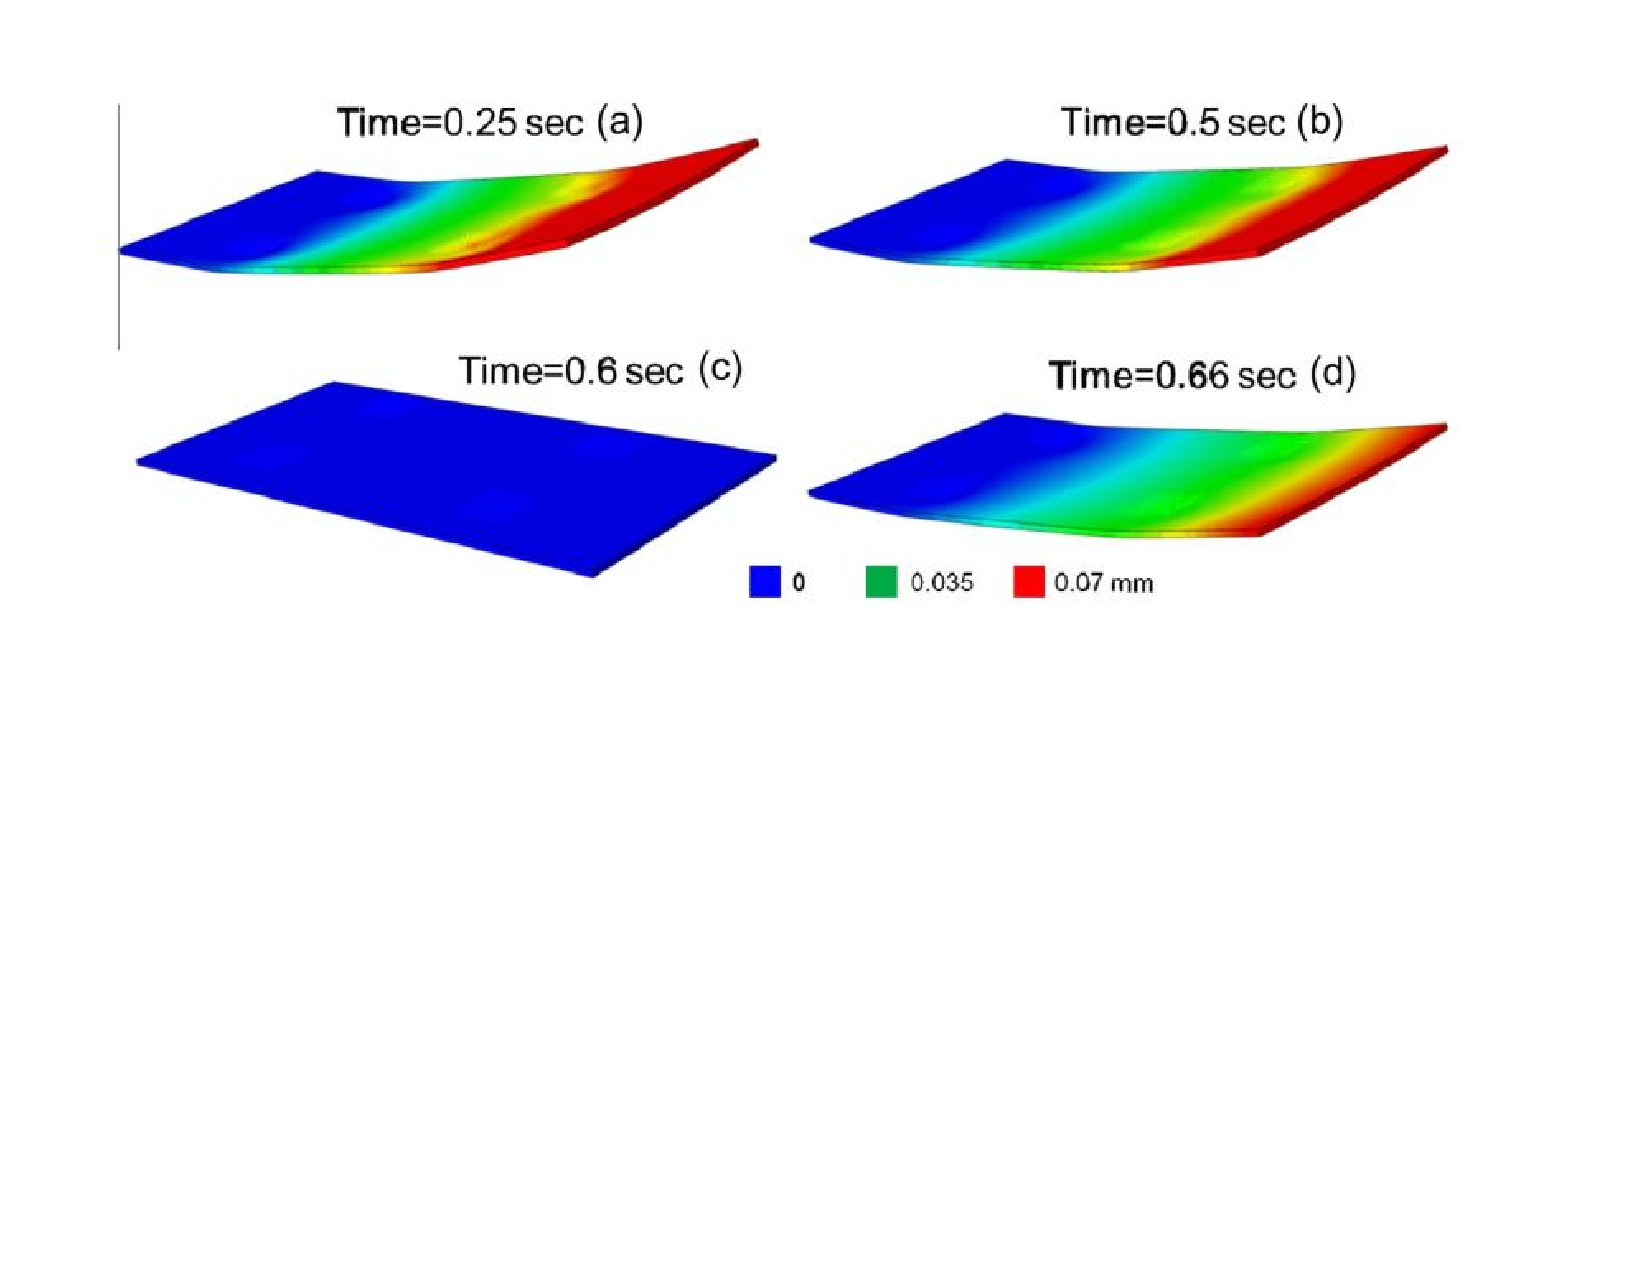
\includegraphics[height=8cm]{../images/active_patched_beam_deflection_contour.pdf}
\caption{Defromed shape of patched beam under sine input}
\end{figure}
\end{frame}

\begin{frame}{Active Fiber Composite}
Active Fiber Composite (AFC) is an actuation architecture that has been introduced to amplify the deflection cased by piezo-electric effect.
It is formed by placing PZT fibers in epoxy matrix. 
\begin{figure}
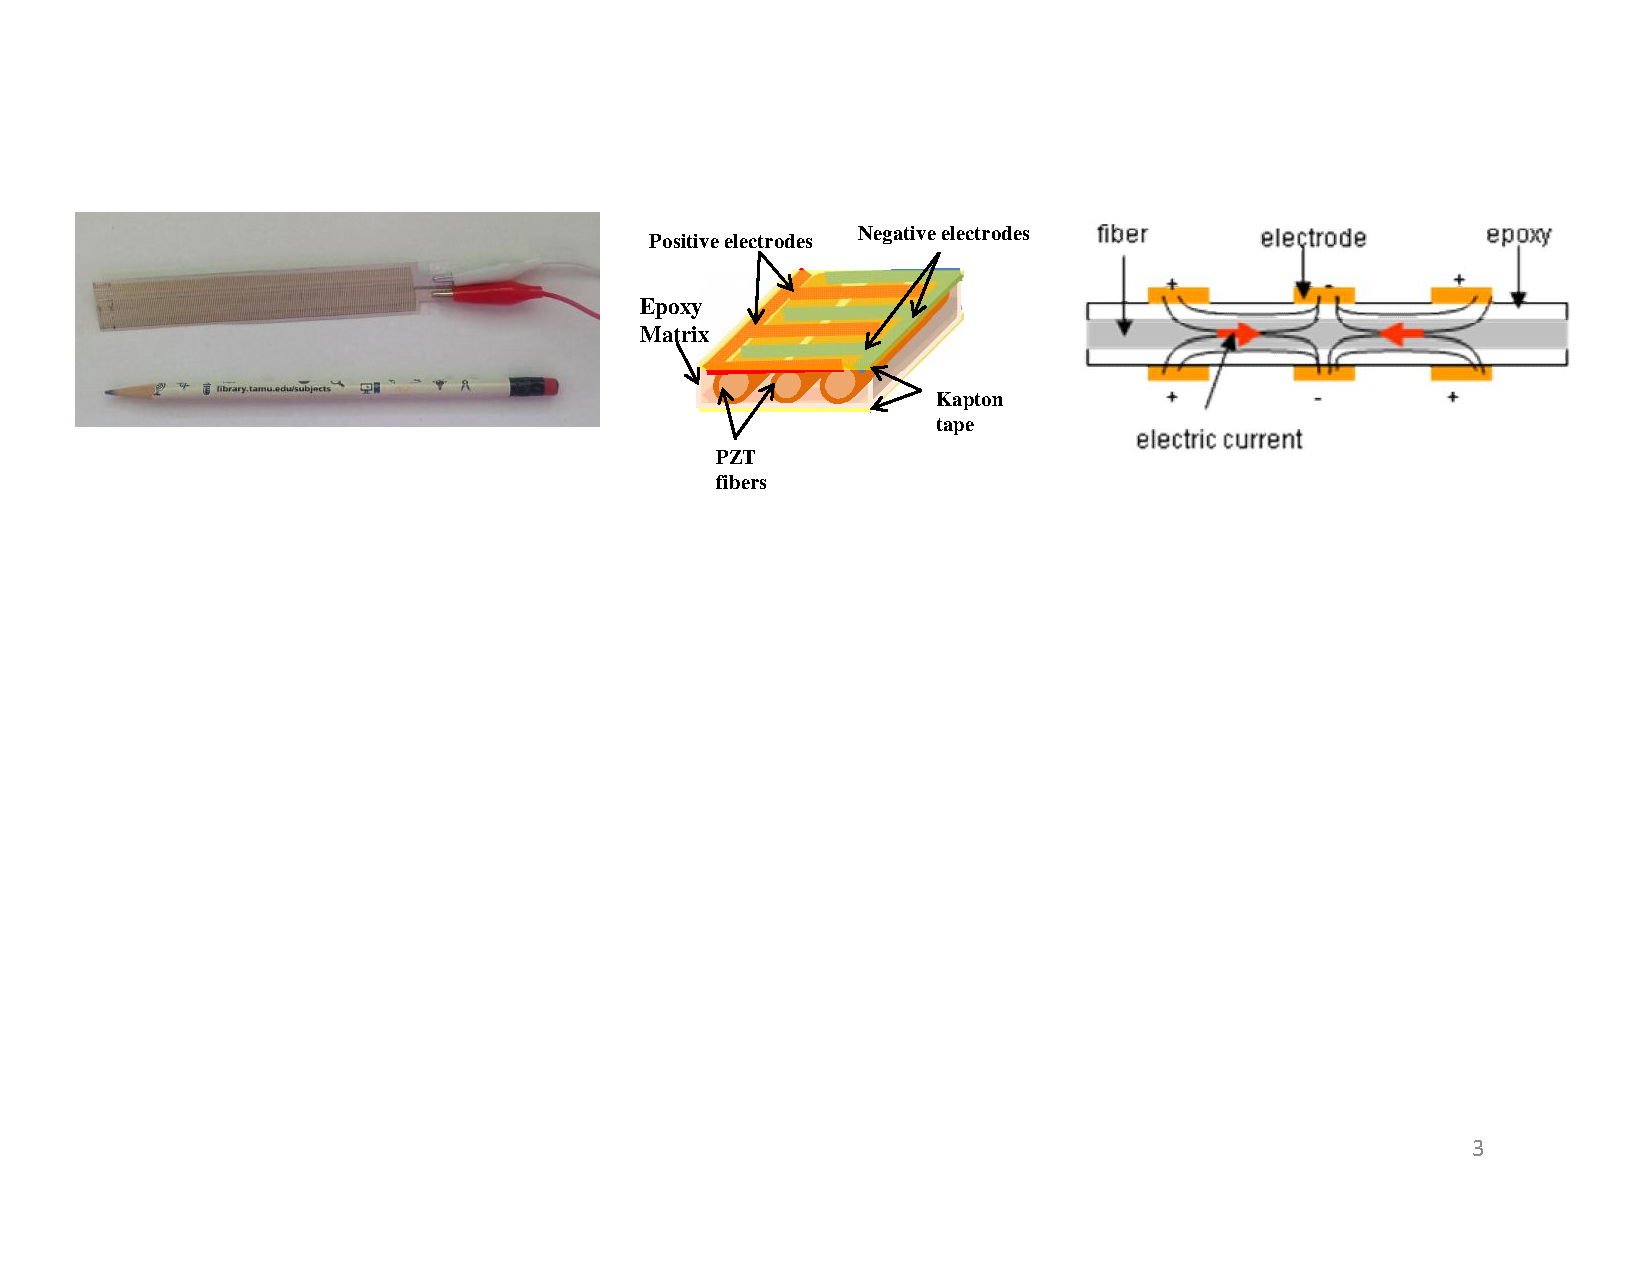
\includegraphics[scale=0.35,trim = 0mm 0mm 0mm 0mm]{../images/active_fiber_composite_pictures.pdf}
\end{figure}
\end{frame}

\begin{frame}{The smallest possible unite cell of AFC is considered in order to simulate the overall performance of AFC.}
Active Fiber Composite (AFC) is an actuation architecture that has been introduced to amplify the deflection cased by piezo-electric effect.
It is formed by placing PZT fibers in epoxy matrix. 
\begin{figure} 
\centering
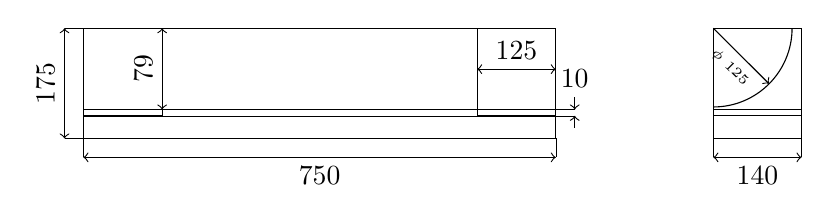
\begin{tikzpicture} [scale=0.80]

\coordinate (a) at (0,0);
\coordinate (b) at (7.50,1.75);

\draw (0,0) rectangle (b) ; 

\draw (0,0.36) rectangle (1.25,0.46);
\draw (6.25,0.36) rectangle (7.50,0.46); 
  
\draw [very thin,-] (0.0,0.46) --  (7.8,0.46);
\draw [very thin,-] (0.0,0.36) --  (7.8,0.36);

% dimension in the middle from top to electrode
\draw [<->] (1.25,0.46) -- (1.25,1.75) node [sloped,midway,above] {79};

% right dimension for  right electrode
\draw  [<-] (7.8,0.46)--(7.8,0.66) node [above]  {10};
\draw  [<-] (7.8,0.36)--(7.8,0.16);

%vertical dimenstion
\draw [<->] (-0.30,0) --  (-0.30,1.75) node [sloped,midway,above] {175};
\draw [very thin,-] (0.0,0) --  (-0.30,0);
\draw [very thin,-] (0.0,1.75) --  (-0.30,1.75);

% horizental dimension of electrode
\draw [very thin,-] (6.25,0.36) -- (6.25,1.75);
\draw [<->] (6.25,1.1) --  (7.5,1.1)  node [sloped,midway,above] {125};

%horizentoal dimenstion
\draw [<->] (0,-0.30) --  (7.50,-0.30) node [sloped,midway,below] {750};
\draw [very thin,-] (0,0) --  (0,-0.30);
\draw [very thin,-] (7.5,0) --  (7.5,-0.30);


%% The left view
\draw (10.0,0) rectangle (11.4,1.75) ; 
%% The horizental dimension
\draw [<->] (10.0,-0.3)--  (11.4,-0.3) node [sloped,midway,below] {140};
\draw [very thin,-] (10.0,0) --  (10.0,-0.3);
\draw [very thin,-] (11.4,0) --  (11.4,-0.3);

%% The fiber
\draw (11.25,1.75) arc  (0:-90:1.25) ; 
%% The electode in the view
\draw (10.0,0.36) rectangle (11.4,0.46) ;

%% The radial dimension
\draw [<-] (10.883,0.8698) -- (10.0,1.75)  node [sloped,midway,below]{\tiny $\phi$ 125};

\end{tikzpicture}
\caption{Geometry of Unit Cell (dimensions are in $\mu m$)}
\label{fig:geometry_unit_cell_afc}
\end{figure}
\end{frame}

\begin{frame}{Result for AFC Unit Cell }
The finite element model for AFC unit cell\\ 
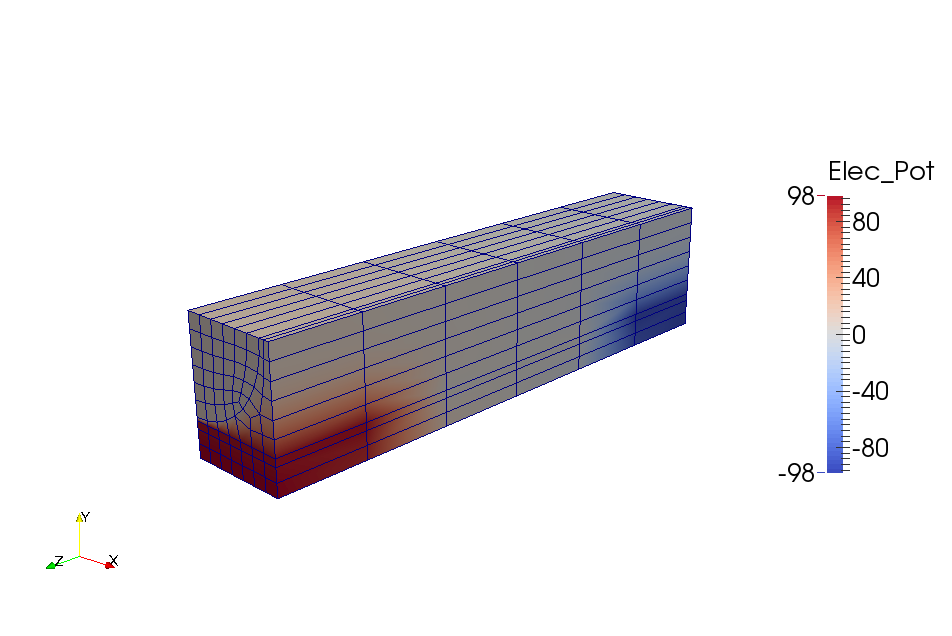
\includegraphics[height=3cm]{../images/afc_epot.png}\\      
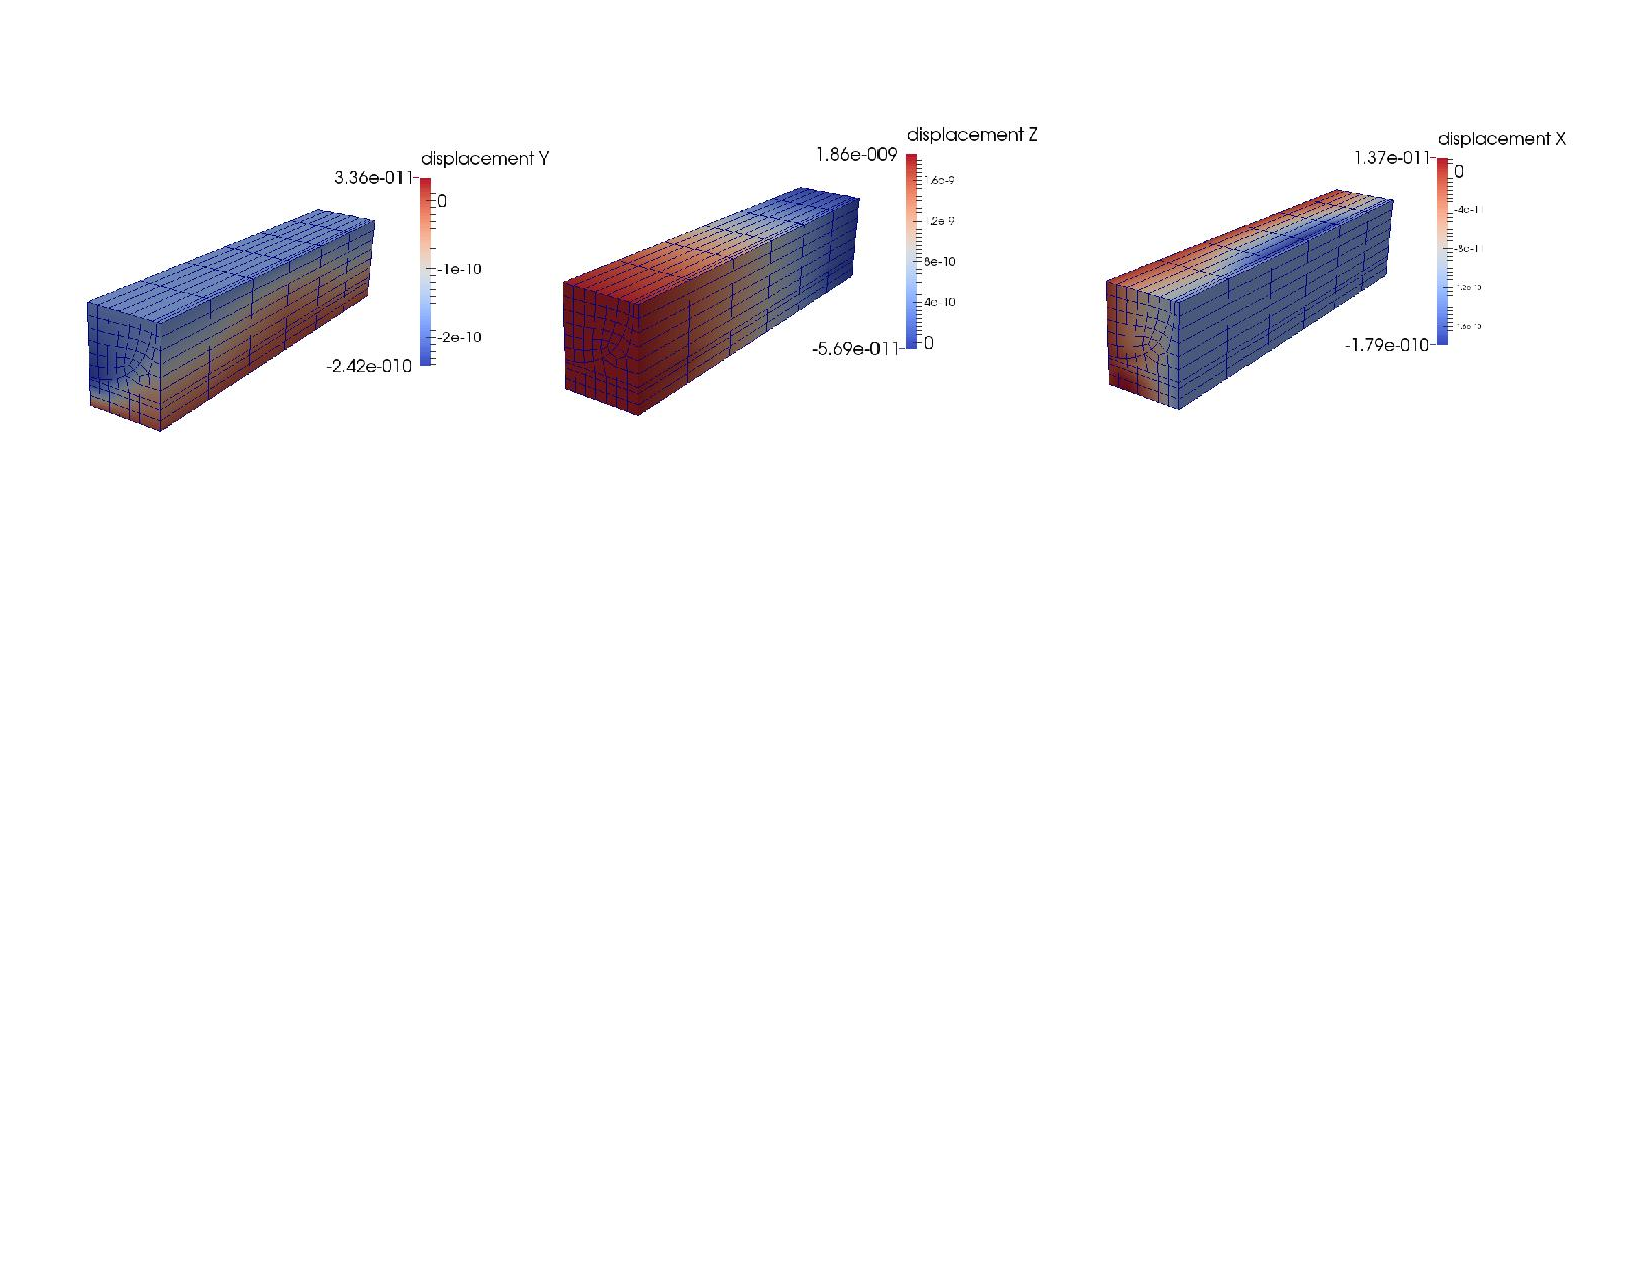
\includegraphics[width=10cm]{../images/afc_displacement_all.pdf}\\  
\end{frame}

\begin{frame}{Large Strain in Elecro Active Polymers}
Electro Active Polymers offering large deformation under large electric fields. 
The total free energy for the EAPs, $\Phi$, is:
\begin{block}<+->{Total Elergy of EAP}
\begin{equation}
\Phi=\Phi_{m}+\Phi_{e}+\Phi_{em}
\label{EQN:TotalEnergy}
\end{equation}
\end{block} 
where $\Phi_{m}$ is the mechanical part and defined as:
\begin{block}{Mechnical Part of Energy $\Phi_{m}$}
\begin{equation}
\Phi_{m}=\frac{\kappa}{2} (J-1)+\frac{\mu}{2} (\overline{\mathbf{C}}:\mathbb{I}-dim)
\label{EQN:eap_mechanical_part}
\end{equation}
\end{block} 
$\kappa$, $\mu$, \small are material constants, \\
$J$, $\overline{\mathbf{C}}$ \small are Jacobian of the deformation gradient
tensor and isochoric part of right Cauchy Green strain tensor
\end{frame}

\begin{frame}{Large Strain in Elecro Active Polymers}
Electromechanical part is defined with respect to electric feild vector
$\mathbf{E}$ and a constant $C_m$
\begin{block}{ElectroMechnical Part of Energy $\Phi_{em}$}
\begin{equation} 
\Phi_{em}=C_m (\overline{\mathbf{C}} : \mathbf{E}\otimes \mathbf{E})
\label{EQN:eap_electromechanical_part}
\end{equation}
\end{block} 

\begin{block}{Purely Electric Part of Energy $\Phi_{e}$}
\begin{equation} 
\Phi_{e}=C_e (\mathbb{I} : \mathbf{E}\otimes \mathbf{E})-\epsilon_0 J \mathbf{C}^{-1} :(\mathbf{E}\otimes \mathbf{E})
\label{EQN:eap_electric_part}
\end{equation}
\end{block} 
$C_e$,$\epsilon_0$ are the electric permitivity of material and permitivity of
free space respectively.

\end{frame}

\begin{frame}{Finite Element Model for Electro Active Polymers}
\begin{block}{The Virtual Work Statement}
\begin{equation} 
\delta \pi=\int_V P_{ij}\delta F_{ij} dV -\int_V D_{i}\delta E_{i}
dV-\int_{\partial V} T_{i}\delta u_{i} d{\partial V}-\int_{\partial V} Q\delta \phi d{\partial V}
\label{EQN:eap_electromechanical_part}
\end{equation}
\end{block} 

\begin{block}{The 1st Piola Kirchhoff stress and electric displacement}
\begin{equation} 
P_{ij}=\frac{\partial \Phi}{\partial F_{ij}} ;D_{i}=-\frac{\partial \Phi}{\partial E_{i}}
\label{EQN:eap_electric_part}
\end{equation}
\end{block} 
\end{frame}

\begin{frame}{Finite Element Model for Electro Active Polymers}

\begin{block}{Gradient of Deformation and Electric Field}
\begin{equation} 
\begin{aligned}
& F_{ij}=\frac{\partial u_i}{\partial X_{i}}+\delta_{ij} \\
& \delta F_{ij}=\frac{\delta \partial u_i}{\delta \partial X_{i}}
&E_{i}=\frac{\partial \psi}{\partial X_{i}}\\
\end{aligned}
\label{EQN:Disp_F_Relation}
\end{equation}
\end{block} 

where $\partial \psi$ is the electric potential.
The finite element model will be developed based on 

\begin{equation}
R_k=\frac{\partial \delta \pi}{\partial \delta d_k}=0 ,(k=1\dots NDF)
\label{EQN:ResidualRepresentation}
\end{equation}

\end{frame}


\begin{frame}

\begin{figure}
\centering
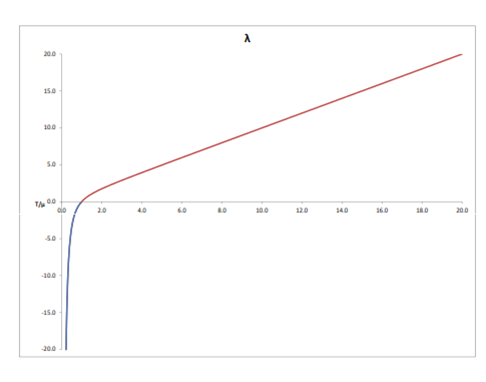
\includegraphics[scale=0.3,trim = 0mm 0mm 0mm
00mm]{../images/eap_stress_stretch.png}
\label{fig:mechanical}
\caption{Mechanical Response}
\end{figure} 
\begin{figure}
\centering
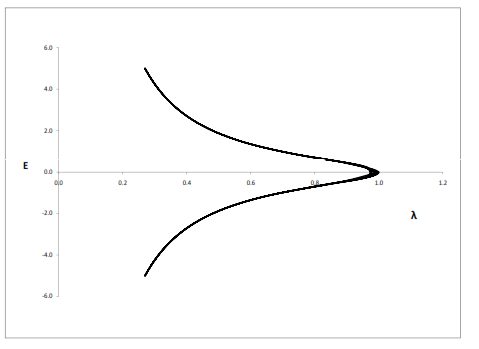
\includegraphics[scale=0.3,trim = 0mm 0mm 0mm
00mm]{../images/eap_elect_stretch.png}
\label{fig:mechanical}

\caption{Electromechanical Response}

\end{figure} 

\end{frame}
\begin{frame}{Conclusion}
\begin{figure}
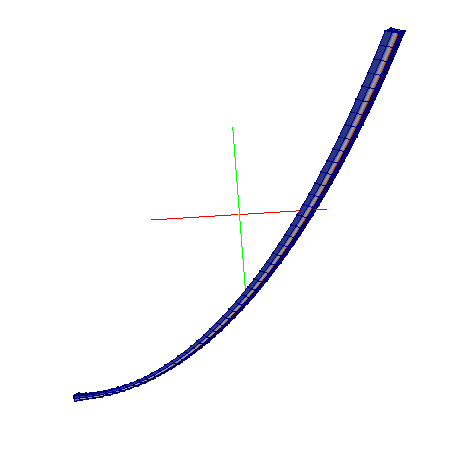
\includegraphics[scale=0.3,trim = 0mm 0mm 0mm
00mm]{../images/EAP_BEAM_EPOT_DEFLECTION.png}
\label{fig:EAP_BEAM}
\caption{Bimorph Electro Active Beam}
\end{figure}
\end{frame}

\subsection{Active Trusses}

\begin{frame}{Active Truss Structure }
In this part of research we will try to find a way to control shape of an active truss system. This system can be embedded into a matrix and offer desired shape for plate or other type of structures

     \begin{columns}[t] % contents are top vertically aligned
     \begin{column}[T]{5cm} % each column can also be its own environment
       \begin{itemize} \itemsep10ex
  \item  Reference Configuration   \\
  \item  Deformed Configuration
  \end{itemize} 
     \end{column}
     \begin{column}[T]{5cm} % alternative top-align that's better for graphics
      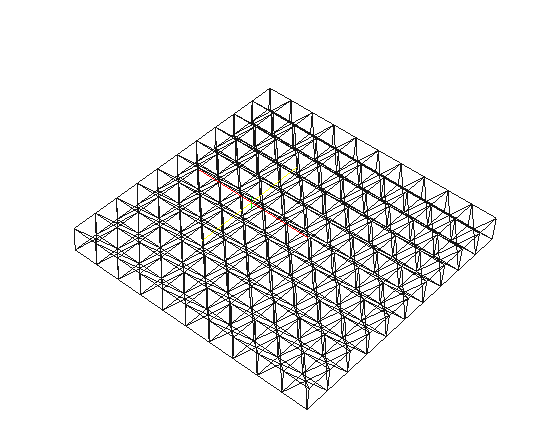
\includegraphics[height=2cm]{../images/Truss_3D_Shape_z_xy_deformation_Undeformed}\\
      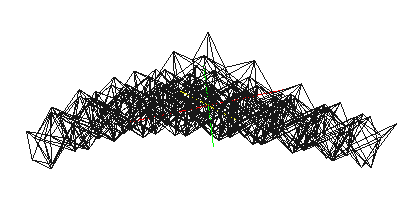
\includegraphics[height=2cm]{../images/Truss_3D_Shape_z_xy_deformation_ZY_Plane}\\     
     \end{column}
     \end{columns}    
\end{frame}


\begin{frame}{Deformation gradient}
\begin{itemize}
\item  Refrence configuration is defined as $X_i$
\item  Deformed configuration is defined as $x_i$
\item  The gradient of deformation will be $F_{ij}=\frac{\partial
x_j}{\partial X_j}$
\item The strain induced due to this change in configuration is 
$E_{KL}=\frac{1}{2}\left( \frac{\partial x_j}{\partial X_K}\frac{\partial x_j}{\partial X_L}-\delta_{KL}\right)$ 
\item  Components of direction vector of truss element are $n^{ele}_i$
\item  The constitutiv equation between two point of the truss
$C_{ijkl}= n^{ele}_i n^{ele}_j n^{ele}_k  n^{ele}_l E_Y$
\end{itemize}      
\end{frame} 


\begin{frame}{Tetrahedral truss}
\begin{itemize}
\item Desired shape
\begin{figure}
\fbox{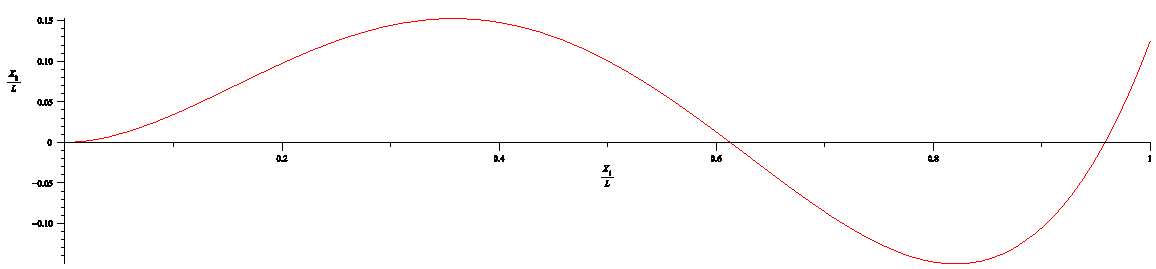
\includegraphics[scale=0.2]{../images/curve_beam-eps-converted-to}}
\end{figure}

\item The applying the shape change stress
\begin{figure}
\fbox{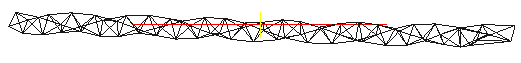
\includegraphics[scale=0.4]{../images/refrence_tetra_beam}}
\fbox{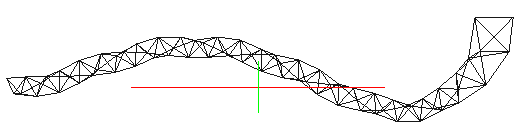
\includegraphics[scale=0.4]{../images/current_tetra_beam}}
\end{figure}
%% 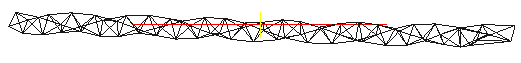
\includegraphics[scale=0.6]{../images/refrence_tetra_beam}
%% 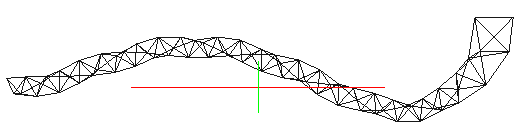
\includegraphics[scale=0.6]{../images/current_tetra_beam}
\end{itemize}
\end{frame}

\begin{frame}{Plane Truss}
\begin{itemize}
\item Desired shape $z=xy$
\begin{figure}  
\fbox{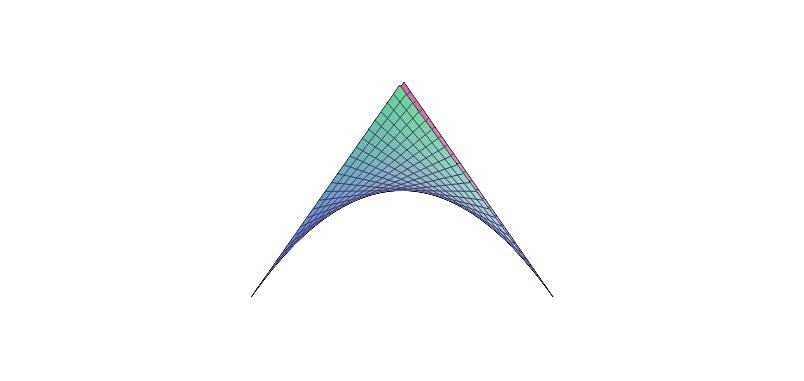
\includegraphics[scale=0.2]{../images/xy_plane_desired_shape}}
\end{figure}

\item The applying the shape change stress
\begin{figure}
\fbox{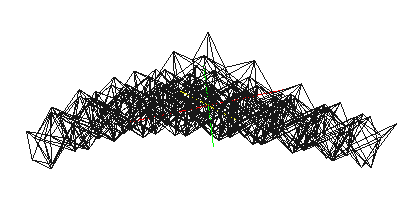
\includegraphics[scale=0.4]{../images/Truss_3D_Shape_z_xy_deformation_ZY_Plane}}
\end{figure}
%% 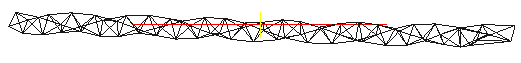
\includegraphics[scale=0.6]{../images/refrence_tetra_beam}
%% 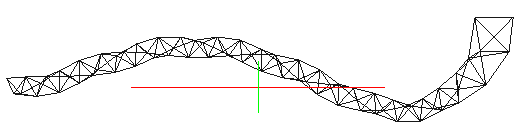
\includegraphics[scale=0.6]{../images/current_tetra_beam}
\end{itemize}
\end{frame}

\begin{frame}{Conclusion}
\begin{itemize}
\item The nonlinear time dependent constitutive equation is  incorporated into FE model
\item The developed FE model is validated by several computational close form solutions and also experimental data
\item Performance of developed model is shown by simulating  active structures
\end{itemize}   
\end{frame}

\begin{frame}
We thank the Air Force Office of Scientific Research (AFOSR) under grant FA 9550-10-1-0002 for sponsoring this research.
\end{frame}


\begin{frame}
Questions
?
\end{frame}


\begin{frame}{References}
\fontsize{8pt}{8pt}
\bibliographystyle{plain}
\bibliography{references}
  
\end{frame}

\end{document}